\chapter[Web et usages sociétaux]{Web et usages sociétaux}
\label{chap:II}

\lettrine{L}{e Web social, aussi connu sous le nom de Web 2.0}, a considérablement transformé les usages de l'Internet. Aujourd'hui, plus d'une dizaine de réseaux sociaux ont dépassé les cent millions d'utilisateurs ; à l'exemple, \textsc{Wikipédia} est une gigantesque encyclopédie élaborée par ses propres utilisateurs. 

Comment le Web a-t-il évolué d'un utilitaire documentaire vers une vocation à caractère social ? Comment ont émergé les réseaux sociaux au cœur du Web 2.0 ? Des chercheurs tentent de répondre à ces questions et modélisent les usages sociaux du Web...

Parmi ces pratiques, devenues naturelles au quotidien pour la plupart\parnote{De nouveau, comme au chapitre précédent, notons que les services et utilisations sociales du Web ont encore aujourd’hui leurs laissés-pour-compte : « fracture numérique » déjà évoquée ou « zones blanches » de certains territoires, entre autres ruraux.} des individus, certaines, comme le « calcul dans les nuages » ou les monnaies cryptographiques, sont peu ou mal connues et méritent d'être mieux appréciées, en particulier dans leurs implications.
\parnotes
%\vspace*{1pt}
\vspace*{2.5\baselineskip}

%L'ensemble de ces considérations et enjeux sont ceux du présent chapitre.

%----------
\section[Web et réseaux sociaux]{Web et réseaux sociaux}
\label{sec:II.1}

Qu'est-ce que le Web ?\caution[t]<secondcolor>{%
\href{http://www-sop.inria.fr/members/Fabien.Gandon/}{Fabien \textsc{Gandon}}, directeur de recherche \textsc{Inria} et responsable de l'équipe \href{https://www.inria.fr/fr/liste-des-equipes-projets}{\textsc{Wimmics}} (Université Côte d’Azur, \textsc{Cnrs} I3S), étudie modèles et algorithmes afin de concilier \href{https://fr.wikipedia.org/wiki/Web_social}{Web social} et \href{https://fr.wikipedia.org/wiki/Web_s\%C3\%A9mantique}{Web sémantique}. Il est aussi représentant de l'\textsc{Inria} au consortium international de standardisation pour le Web (\href{https://www.w3.org/}{W3C}).}{À propos de l'intervenant}
Plutôt que le définir directement, il peut être plus aisé de répondre à son contraire : qu'est-ce que le Web n'est pas ? Cette approche se justifie notamment parce que les gens font souvent l'amalgame entre \gls{web} et \gls{internet}. Ainsi, le Web n'est pas l'Internet. 

L'Internet est en effet un ensemble de standards et de technologies qui permettent de relier des ordinateurs et de raccorder des réseaux entre eux. On peut le concevoir comme un réseau routier sur lequel vont transiter différents types de services, de marchandises, de personnes ou encore de véhicules.

À l'instar du réseau routier offrant le passage de multiples éléments, l'Internet est le support de divers types d'application. Dans cette assertion, le Web en est une parmi d'autres.


%\vspace*{-0.5pt}
\subsection[Avènement du Web social]{Avènement du Web social}
\label{sub:II.1.1}

Le Web n'est clairement pas le seul «~objet~» de l'Internet. On peut par exemple également citer le courrier électronique, la téléphonie --- \textsc{VoIP}, \textit{Voice over Internet Protocol} --- ou plus récemment la télévision et, plus largement, le multimédia. Il faut donc bien distinguer entre cette infrastructure de réseaux reliés entre eux que représente l'Internet et une de ses applications en surcouche qu'est le Web (protocole \texttt{http}). 

\begin{marginvideo}
	[\label{vid:II.1}Web sociétal I.]%
	%\includemedia[
	%	addresource=./Videos/Chapter01/vidI-01-umount-computer-HD.mp4,
	%	%width=0.6\linewidth, height=0.3375\linewidth, % 16:9
	%	flashvars={source=./Videos/Chapter01/vidI-01-umount-computer-HD.mp4&scaleMode=letterbox}
	%	]%
	%	{
\includegraphics[scale=0.75]{./Images/Pictograms/film-strip-red-brown.png}}{StrobeMediaPlayback.swf}
	%\movie[width=\marginparwidth,showcontrols]%
	%	{
\includegraphics[width=\marginparwidth]{./Images/Pictograms/film-strip-dark-electric-blue.png}}%
	%	{./Videos/Chapter02/vidII-01-socialweb-01-HD.mp4}%
	\href{https://www.youtube.com/watch?v=Tt7dat0QbbE&list=PLWvGMqXvyJAMNWRvODUB5Ry3licACdaa0&index=11}%
		{
\includegraphics[width=\marginparwidth]{./Images/Pictograms/film-strip-dark-electric-blue.png}}%
	\launchvideo{https://www.youtube.com/watch?v=Tt7dat0QbbE&list=PLWvGMqXvyJAMNWRvODUB5Ry3licACdaa0&index=11}
\end{marginvideo}


\subsubsection[\textit{World Wide Web}]{\textit{World Wide Web}}
\label{subsub:II.1.1.1}

Initialement, le Web en lui-même est développé comme une application dévolue au partage d'une information statique, texte et image. Ces prémisses se situent au \textsc{Cern} --- à la frontière franco-suisse --- et datent du tournant des décennies 1980-1990. L'idée est alors d'apparier des documents entre eux pour permettre leur accès, même s'ils ne résident pas physiquement sur la même machine. 

Au début, l'usage de cette fonctionnalité est réservée aux scientifiques, suite à l'ouverture progressive des connexions des universités à l'Internet --- en France, avec \textsc{Renater} pour RÉseau NAtional de Télécommunications pour la Technologie, l'Enseignement et la Recherche.

Au cours des années 1990, l'offre s'élargit assez rapidement au grand public. De ce point de vue, l'année 1997 marque en France un moment décisif : à la fois une meilleure accessibilité des matériels en termes de coût --- ordinateur personnel (\textsc{Pentium} premières générations) et modem (modulateur-démodulateur) ---, autant que les premières offres de service des fournisseurs\sidenote{À titre de comparaison et en référence au chapitre précédent, on remarque que \textsc{Linux} a vu son lancement en 1991, connu sa première phase de stabilisation de 1992 à 1996 pour fournir une solution viable au technophile moyen. Cette évolution s'est réalisée à travers le réseau téléphonique commuté au moyen de modems permettant 56 bauds de vitesse de transmission\linebreak théorique. Le prix des mémoires et transfert de données de cette époque imposait derechef une optimisation des codes.} d'accès à l'Internet (\textsc{FAI}).

Le Web devient alors littéralement cette \emph{toile} mondiale. En même temps, cela s'avère un peu ambigu puisque c'est à la fois les standards d'Internet qui permettent de créer cet objet et celui qui en émerge ; la toile mondiale sur laquelle on se balade tous les jours. 

Dès l'origine de la « toile » dûment nommée, deux facettes se présentent. La première est d'ordre documentaire, afin d'associer des documents résidant potentiellement sur différentes machines. Mais il y a également l'idée que de multiples personnes puissent contribuer à différents documents demeurant sur plusieurs serveurs. Dès le départ, ces deux aspects --- documentaire et social --- coexistent, en perspective d'une interaction entre les divers contributeurs. 

Au début, le Web est ouvert en écriture, mais très peu utilisent cette possibilité. La plupart des premiers serveurs Web sont accédés en lecture. Il faut attendre le milieu des années 1990 et la réouverture du Web en écriture notamment avec les \textit{wikis} pour avoir la possibilité de voir tout le monde contribuer. C'est vraiment à ce moment-là que l'on bascule vers le Web social et toutes les applications sociales que l'on connaît désormais sur le Web.

\subsubsection[Réseaux sociaux]{Réseaux sociaux}
\label{subsub:II.1.1.2}

\sidegraphic{%

\includegraphics[width=0.75\linewidth]{linkedIn-logo.pdf}\\[16pt]

\includegraphics[width=0.75\linewidth]{facebook-logo-full.pdf}%
}%
Les \glspl{social-network} prennent de multiples formes, mais on peut énoncer la définition d'un réseau social telle que celle proposée actuellement dans la presse : une application qui va utiliser les sciences et technologies de l'information, donc le Web, Internet et autres appareils mobiles pour mettre en \gls{link} des personnes. Cela constitue leur tronc commun depuis lequel elles se différencient, notamment en termes d'usage. 
S'agit de relier entre eux des \textit{curriculum vitæ} sur \textsc{LinkedIn} ou d'échanger des messages plus ou moins sérieux sur \textsc{Facebook}.

Ces applications diffèrent également en type de liens dans le réseau. Par exemple, est-ce un réseau d'amis, professionnel ou fondé sur des centres d'intérêt ? Une autre différenciation est aussi recouverte par les moyens d'accès : à travers le Web avec un navigateur sur ordinateur ou un mobile suffit-il. 
La distinction \nopagebreak peut encore s'opérer selon les contenus partagés, \pagebreak à l'instar de messages courts comme sur \textsc{Twitter} ou de vidéos tel que sur \textsc{YouTube}. Ce dernier exemple évoque une catégorie spécifique, le média social. Sa particularité est de produire et d'échanger des contenus multimédias (cf. chaînes \textsc{YouTube}).

\sidegraphic{%

\includegraphics[width=0.3333\linewidth]{twitter-logo.pdf}\\[16pt]

\includegraphics[width=0.3333\linewidth]{youtube-logo.pdf}\\[16pt]

\includegraphics[width=0.3333\linewidth]{researchgate-logo-letters.pdf}\\[16pt]

\includegraphics[width=0.45\linewidth]{whatsapp-logo.pdf}\\[16pt]

\includegraphics[width=0.3333\linewidth]{snapchat-logo.pdf}%
}%
On peut aussi mentionner des réseaux sociaux explicites, autrement dit des réseaux sur lesquels les différents types de liens avec les autres personnes sont activement déclarés (cf. \textsc{LinkedIn}), avec des réseaux sociaux qu'on peut qualifier d'implicites, c'est-à-dire dont la relation est calculée par rapport à l'activité des utilisateurs. 
En sciences, il existe des applications sociales comme \textsc{ResearchGate} qui permettent aux scientifiques de poster et de maintenir leur bibliographie et les articles qu'ils écrivent. À travers cette activité et en regardant quelles sont leurs coauteurs, on peut en déduire un réseau social implicite à cette activité. 
Enfin, une discrimination peut se conduire selon la plateforme : les applications sont-elles définitivement ancrées sur le Web comme \textsc{Tumblr} où associées aux réseaux mobiles telles \textsc{WhatsApp} ou \textsc{Snapchat} ?

%Donc en fait pour conclure, on pourrait dire que grosso modo on a à la fois un tronc commun qui est cette idée que ce sont des applications qui utilisent les nouvelles technologies de l'information pour mettre des liens entre les personnes, pour permettre de créer des liens entre personnes. Et en même temps, elles ont un ensemble de différences à travers leurs usages, les types de contenus, les types de liens qu'elles permettent de créer.

Par ailleurs, les réseaux sociaux n'ont pas attendu Internet ni même l'informatique pour exister. Depuis très longtemps la notion de structures sociales est étudiée en sociologie ; posséder et disposer d'un réseau est une expression bien connue.
Même en informatique, cela prédate Internet. En fait, les \href{https://fr.wikipedia.org/wiki/Bulletin_board_system}{\textit{Bulletin Boards Systems} (BBS)} ont connu leur apogée avant Internet dans les années 1970. Dans la foulée, des applications comme \href{https://fr.wikipedia.org/wiki/Usenet}{\textit{Usenet}} et les \textit{Newsgroups} ont pris le relai sans attendre le déploiement complet de l'Internet. Dans la continuité, on va avoir le courriel avec les \textit{mailing lists}, mais également les IRC --- \textit{Internet Relay Chat} --- pour les conversations synchronisées. Ainsi, les forums ou \textit{chat rooms} --- salles de discussion --- commencent très tôt en informatique.

Ensuite, avec le déploiement d'Internet, mais surtout du Web, cet espace n'est plus réservé aux technophiles. 
Une bascule s'opère en effet dans les années 1990 parce que le Web non seulement démocratise l'accès à Internet, mais aussi devient social. C'est-à-dire que ce n'est plus une bibliothèque, mais un endroit où tout le monde va pouvoir contribuer et écrire. 
Au début, c'est assez simple comme avec \textsc{Six Degrees} ou \textsc{Classroom} pour simplement dire qui était son camarade de classe avant. Puis, petit à petit, apparaissent des applications comme les \textit{wikis}, les \textit{forums}, les \textit{blogs} qui vont inviter à la contribution et donc aux médias sociaux.  


\begin{marginvideo}
	[\label{vid:II.2}Web sociétal II.]%
	%\includemedia[
	%	addresource=./Videos/Chapter01/vidI-01-umount-computer-HD.mp4,
	%	%width=0.6\linewidth, height=0.3375\linewidth, % 16:9
	%	flashvars={source=./Videos/Chapter01/vidI-01-umount-computer-HD.mp4&scaleMode=letterbox}
	%	]%
	%	{
\includegraphics[scale=0.75]{./Images/Pictograms/film-strip-red-brown.png}}{StrobeMediaPlayback.swf}
	\href{https://www.youtube.com/watch?v=iex5zjJEuzs&list=PLWvGMqXvyJAMNWRvODUB5Ry3licACdaa0&index=12}%
		{
\includegraphics[width=\marginparwidth]{./Images/Pictograms/film-strip-dark-electric-blue.png}}%
	%\movie[width=\marginparwidth,showcontrols]%
	%	{
\includegraphics[width=\marginparwidth]{./Images/Pictograms/film-strip-dark-electric-blue.png}}%
	%	{./Videos/Chapter02/vidII-01-socialweb-02-HD.mp4}%
	\launchvideo{https://www.youtube.com/watch?v=iex5zjJEuzs&list=PLWvGMqXvyJAMNWRvODUB5Ry3licACdaa0&index=12}
\end{marginvideo}

\subsubsection[Modélisation]{Modélisation des réseaux sociaux}
\label{subsub:II.1.1.3}

Quand on a besoin de représenter ou de modéliser les réseaux en mathématiques, en informatique et plus généralement en sciences du numérique, le premier type de modèle employé se réfère à la \href{https://fr.wikipedia.org/wiki/Th\%C3\%A9orie_des_graphes}{\emph{théorie des graphes}}, pour capturer la structure du réseau social. 

\sidefigure[\label{fig:II.1}Réseaux et graphes.]{%
\begin{tikzpicture}[scale=1.0, >=latex, inner sep=0pt, outer sep=0pt, label distance=2pt]
%\draw[step=0.25cm,style=help lines, line width=0.1pt] (-2.5,-3) grid (2.5,3);
%\draw[step=1cm,style=help lines, line width=0.6pt] (-2.5,-3) grid (2.5,3);
%-----
\draw[bend right] (-1.25,-0.5) to node[font=\tiny, auto, swap, inner sep=1pt] {ami} (-2.0,0.5);
\node[label=left:{\scriptsize Franck}] at (-1.25,-0.5) {\faUser};
\node[label=right:{\scriptsize Laurence}] at (-2.0,0.5) {\faUser};
\draw[bend left] (-2.0,0.5) to node[font=\tiny, auto, inner sep=1pt] {ami} (-1.75,2.0);
\node[label=left:{\scriptsize Rose}] at (-1.75,2.0) {\faUser};
\draw[bend left] (-2.0,0.5) to node[font=\tiny, auto, inner sep=1pt] {sœur} (-1.0,1.25);
\node[inner sep=0pt, outer sep=0pt, label=below:{\scriptsize Thomas}] at (-1.0,1.25) {\faUser};
\draw[bend left] (-1.75,2.0) to node[font=\tiny, auto, inner sep=1pt] {ami} (-0.25,2.25);
\draw[bend left] (-1.0,1.25) to node[font=\tiny, auto, inner sep=1pt] {marié} (-0.25,2.25);
\draw[bend right] (-1.0,1.25) to (-0.25,2.25);
\node[label=above:{\scriptsize Stéphanie}] at (-0.25,2.25) {\faUser};
\draw[bend left] (-0.25,2.25) to node[font=\tiny, auto, inner sep=1pt] {sœur} (1.0,2.0);
\node[label=right:{\scriptsize Joséphine}] at (1.0,2.0) {\faUser};
\draw[bend right] (1.0,2.0) to node[font=\tiny, auto, swap, inner sep=1pt] {parent} (0.5,0.5);
\draw[bend left] (1.0,2.0) to node[font=\tiny, auto, inner sep=1pt] {parent} (1.5,0.5);
\node[label=below:{\scriptsize Éric}] at (0.5,0.5) {\faUser};
\node[label=below:{\scriptsize Amélie}] at (1.5,0.5) {\faUser};
\end{tikzpicture}%
}

%--- BUG: NO AUTOMATIC DETECTION BUT IT WORKS WITH \sidefigure!!! WHY???
%\begin{marginfigure}
%\begin{tikzpicture}[scale=1.0, >=latex, inner sep=0pt, outer sep=0pt, label distance=2pt]
%%\draw[step=0.25cm,style=help lines, line width=0.1pt] (-2.5,-3) grid (2.5,3);
%%\draw[step=1cm,style=help lines, line width=0.6pt] (-2.5,-3) grid (2.5,3);
%%-----
%\draw[bend right] (-1.25,-0.5) to node[font=\tiny, auto, swap, inner sep=1pt] {ami} (-2.0,0.5);
%\node[label=left:{\scriptsize Franck}] at (-1.25,-0.5) {\faUser};
%\node[label=right:{\scriptsize Laurence}] at (-2.0,0.5) {\faUser};
%\draw[bend left] (-2.0,0.5) to node[font=\tiny, auto, inner sep=1pt] {ami} (-1.75,2.0);
%\node[label=left:{\scriptsize Rose}] at (-1.75,2.0) {\faUser};
%\draw[bend left] (-2.0,0.5) to node[font=\tiny, auto, inner sep=1pt] {sœur} (-1.0,1.25);
%\node[inner sep=0pt, outer sep=0pt, label=below:{\scriptsize Thomas}] at (-1.0,1.25) {\faUser};
%\draw[bend left] (-1.75,2.0) to node[font=\tiny, auto, inner sep=1pt] {ami} (-0.25,2.25);
%\draw[bend left] (-1.0,1.25) to node[font=\tiny, auto, inner sep=1pt] {marié} (-0.25,2.25);
%\draw[bend right] (-1.0,1.25) to (-0.25,2.25);
%\node[label=above:{\scriptsize Stéphanie}] at (-0.25,2.25) {\faUser};
%\draw[bend left] (-0.25,2.25) to node[font=\tiny, auto, inner sep=1pt] {sœur} (1.0,2.0);
%\node[label=right:{\scriptsize Joséphine}] at (1.0,2.0) {\faUser};
%\draw[bend right] (1.0,2.0) to node[font=\tiny, auto, swap, inner sep=1pt] {parent} (0.5,0.5);
%\draw[bend left] (1.0,2.0) to node[font=\tiny, auto, inner sep=1pt] {parent} (1.5,0.5);
%\node[label=below:{\scriptsize Éric}] at (0.5,0.5) {\faUser};
%\node[label=below:{\scriptsize Amélie}] at (1.5,0.5) {\faUser};
%\end{tikzpicture}
%\caption{\label{fig:II.1}Réseaux et graphes.}
%\end{marginfigure}

Dans un \gls{graph}, on trouve des \emph{nœuds} qui représentent des entités comme les personnes et des \emph{arcs} qui symbolisent les liens entre ces personnes. À partir de là, on va très vite voir que ce modèle peut s'enrichir et qu'émergent différents types de graphes pour décrire divers types de réseaux sociaux (cf. \cref{fig:II.1}).

Si dans un réseau social, plusieurs liens sont possibles entre les personnes --- par exemple un lien familial et un lien professionnel --- le graphe va évoluer vers le multigraphe, c'est-­à-­dire que plusieurs arcs vont relier deux mêmes nœuds.

On peut également faire appel à des \emph{\glspl{oriented-graph}} où les relations entre individus sont dirigées dans un sens déterminé. Avec \textsc{Twitter}, il est possible de suivre les \textit{posts} d'une personne, mais rien n'oblige cette dernière à la réciproque ; les graphes sont alors orientés. Ce n'est pas nécessaire dans le cas de \textsc{Facebook} où la relation « d'amitié » est convenue par défaut comme étant symétrique.

Plusieurs types de liens sont aussi envisageables dans un réseau. \textsc{LinkedIn} propose un lien principal comme étant professionnel, mais il peut y en avoir d'autres. Auquel cas, il sont mentionnés dans un \emph{\gls{labeled-graph}} (voir \cref{fig:II.1}), où les arcs comportent le type de lien entre les sujets.
On peut encore s'intéresser à représenter des communautés ; on ne regarde alors plus vraiment la structure du réseau social, mais plutôt des groupes d'individus en son sein, par exemple selon des critères de mêmes centres d'intérêt. 

\begin{marginfigure}
\begin{subfigure}{\linewidth}
\centering
\begin{tikzpicture}[scale=1.0, >=latex, inner sep=0pt, outer sep=0pt, label distance=2pt]
%\draw[step=0.25cm,style=help lines, line width=0.1pt] (-2.5,0.0) grid (2.5,3.5);
%\draw[step=1cm,style=help lines, line width=0.6pt] (-2.5,0.0) grid (2.5,3.5);
\draw[bend right] (-1.25,-0.5) to node[font=\tiny, auto, swap, inner sep=1pt] {0,9} (-2.0,0.5);
\node[label=left:{\scriptsize Franck}] at (-1.25,-0.5) {\faUser};
\node[label=right:{\scriptsize Laurence}] at (-2.0,0.5) {\faUser};
\draw[bend left] (-2.0,0.5) to node[font=\tiny, auto, inner sep=1pt] {0,7} (-1.75,2.0);
\node[label=left:{\scriptsize Rose}] at (-1.75,2.0) {\faUser};
\draw[bend left] (-2.0,0.5) to node[font=\tiny, auto, inner sep=1pt] {0,9} (-1.0,1.25);
\node[inner sep=0pt, outer sep=0pt, label=below:{\scriptsize Thomas}] at (-1.0,1.25) {\faUser};
\draw[bend left] (-1.75,2.0) to node[font=\tiny, auto, inner sep=1pt] {0,8} (-0.25,2.25);
\draw[bend left] (-1.0,1.25) to node[font=\tiny, auto, inner sep=1pt] {0,5} (-0.25,2.25);
\draw[bend right] (-1.0,1.25) to (-0.25,2.25);
\node[label=above:{\scriptsize Stéphanie}] at (-0.25,2.25) {\faUser};
\draw[bend left] (-0.25,2.25) to node[font=\tiny, auto, inner sep=1pt] {0,1} (1.0,2.0);
\node[label=right:{\scriptsize Joséphine}] at (1.0,2.0) {\faUser};
\draw[bend right] (1.0,2.0) to node[font=\tiny, auto, swap, inner sep=1pt] {0,8} (0.5,0.5);
\draw[bend left] (1.0,2.0) to node[font=\tiny, auto, inner sep=1pt] {0,9} (1.5,0.5);
\node[label=below:{\scriptsize Éric}] at (0.5,0.5) {\faUser};
\node[label=below:{\scriptsize Amélie}] at (1.5,0.5) {\faUser};
\end{tikzpicture}
\caption{\label{fig:II.2a}Graphe pondéré.}
\end{subfigure}
\begin{subfigure}{\linewidth}
\centering
\vspace{4pt}
\scriptsize
\begin{tabular}{@{}c@{~~~~~~}c@{~~~~~~}c@{~~~~~~}c@{~~~~~~}c@{~~~~~~}c@{~~~~~~}c@{~~~~~~}c@{~~~~~~}c@{}}
	& F & L & T & R & S & J & É & A \\
F & 0 & 1 & 0 & 0 & 0 & 0 & 0 & 0 \\
L & 1 & 0 & 1 & 1 & 0 & 0 & 0 & 0 \\
T & 0 & 1 & 0 & 0 & 1 & 0 & 0 & 0 \\
R & 0 & 1 & 0 & 0 & 1 & 0 & 0 & 0 \\
S & 0 & 0 & 1 & 1 & 0 & 1 & 0 & 0 \\
J & 0 & 0 & 0 & 0 & 1 & 0 & 1 & 1 \\
É & 0 & 0 & 0 & 0 & 0 & 1 & 0 & 0 \\
A & 0 & 0 & 0 & 0 & 0 & 1 & 0 & 0 
\end{tabular}
\caption{\label{fig:II.2b}Matrice d’adjacence non pondérée.}
\end{subfigure}
\begin{subfigure}{\linewidth}
\centering
\vspace{4pt}
\scriptsize
\begin{tabular}{@{}c@{~~~~}c@{~~~~}c@{~~~~}c@{~~~~}c@{~~~~}c@{~~~~}c@{~~~~}c@{~~~~}c@{}}
	& F & L & T & R & S & J & É & A \\
F & 0 & 0,9 & 0 & 0 & 0 & 0 & 0 & 0 \\
L & 0,9 & 0 & 0,9 & 0,7 & 0 & 0 & 0 & 0 \\
T & 0 & 0,9 & 0 & 0 & 0,5 & 0 & 0 & 0 \\
R & 0 & 0,7 & 0 & 0 & 0,8 & 0 & 0 & 0 \\
S & 0 & 0 & 0,5 & 0,8 & 0 & 0,1 & 0 & 0 \\
J & 0 & 0 & 0 & 0 & 0,1 & 0 & 0,8 & 0,9 \\
É & 0 & 0 & 0 & 0 & 0 & 0,8 & 0 & 0 \\
A & 0 & 0 & 0 & 0 & 0 & 0,9 & 0 & 0 
\end{tabular}
\caption{\label{fig:II.2c}Matrice d’adjacence pondérée.}
\end{subfigure}
\caption{\label{fig:II.2}Matrices d’adjacence.}
\end{marginfigure}

D'un point de vue mathématique, là où on utilise des graphes, on peut aussi bien employer d'autres structures de modélisation comme les matrices. Une matrice peut s'élaborer à partir d'un graphe, notamment ce qu'on appelle une \emph{\gls{adjacency-matrix}}, c'est-­à-­dire que pour chaque arc présent dans un graphe, pour chaque lien dans le réseau social, le coefficient de la matrice est mis à $1$ pour signifier qu'il existe une relation. Les colonnes et les lignes d'une matrice d'adjacence représentent tous les nœuds du réseau et s'il y a un lien entre deux nœuds le coefficient à l'intersection de la colonne et de la ligne correspondante est mis à $1$, sinon il est à zéro (cf. \cref{fig:II.2b}). 

Ce modèle matriciel peut être amené à évoluer. Si on doit évaluer la force d'une relation interpersonnelle ou tenir compte de sa certitude, en lieu et place d'un système binaire, on peut introduire des coefficients de pondération compris entre $0$ et $1$ : $0,$$25$ pour une relation « faible » ou $0,$$75$ pour un lien relativement fort (voir \cref{fig:II.2c}).

Ainsi, selon le réseau, on est amené à employer diverses modélisations, mais celles-ci sont aussi guidées par les traitements à opérer.



\subsubsection[Enjeux]{Enjeux technoscientifiques}
\label{subsub:II.1.1.4}

Les enjeux technoscientifiques sont nombreux avec les réseaux sociaux ; comme évoqué précédemment, celui du modèle en est déjà un. Viennent ensuite des questions pratiques : comment ce modèle peut être implémenté de façon efficiente en machine pour prendre le moins d'espace possible, pour être indexé et permettre un accès le plus efficace possible ? Mais aussi, comment peut-on le distribuer sur plusieurs machines lorsqu'il devient trop imposant et qu'il ne tient plus sur une seule machine ? 

Donc, les approches de modèle, de représentation, de stockage et de gestion des données posent des interrogations technoscientifiques. En informatique, il y a toujours deux aspects, la structure de données et l'algorithme, émerge alors le problème des traitements à conduire sur les données, qui peuvent s'avérer extrêmement complexes. 

La complexité des traitements tient d'une part, au volume de données à considérer --- certains réseaux sociaux impliquent aujourd'hui des milliards de relations --- et, d'autre part, à la nature même des traitements envisagés sur les données.

Par exemple, il est traditionnel de déterminer le plus court chemin entre deux personnes pour connaître comment elles sont reliées. Cette opération est déjà assez complexe : repérer tous les chemins qui existent, parmi ceux-ci regarder ceux qui concernent les deux nœuds d'intérêt et enfin trouver le plus petit dans cet ensemble. 

De plus, dans un réseau social, on cherche les personnes les plus centrales, autrement dit les plus influentes. Pour cela, il existe une métrique qu'on appelle la \emph{\gls{intermediation}}. Elle consiste à évaluer le nombre de fois où une personne fait partie du plus court chemin entre deux autres. On calcule ainsi à quel point elle est intermédiaire et le nombre de fois où on passe par elle pour relier les autres. Il faut ainsi mesurer tous les plus courts chemins où elles apparaissent. 

On voit là l'augmentation de la complexité des calculs. En combinant celle-ci au volume de données à traiter, on aboutit rapidement à des problématiques d'optimisation des calculs, voire même d'approximation pour obtenir des résultats peut-être pas tout à fait exacts, mais suffisamment corrects et obtenus dans un délai raisonnable.

Plein d'autres questionnements sont à considérer, notamment ceux qui concernent les graphes. Ces derniers sont susceptibles de changer dans le temps en fonction de l'évolution des réseaux sociaux : création comme suppression de relations. Comment gérer, représenter et analyser ces modifications ? En référence aux médias sociaux, comment également traiter les changements de contenus : textes, images, sons, vidéos, etc.

Au global, la problématique est pluridisciplinaire, faisant appel au juridique, au politique et au sociétal. En résumé, on pourrait formuler que c'est justement parce qu'ils sont sociaux que ces réseaux interrogent toutes les disciplines.

\printlocalglossary{7}

\vfill\pagebreak


\subsection[Filtrage selon \textsc{Facebook}]{Algorithme \textit{Edge Rank} ou le filtrage selon \textsc{Facebook}}
\label{sub:II.1.2}

Si vous êtes adepte du réseau social \textsc{Facebook},\caution[t]<firstcolor>{%
Texte rédigé par Rachid \textsc{Guerraoui} et publié sur \href{https://interstices.info/lalgorithme-edge-rank-ou-le-filtrage-selon-facebook/}{Interstices} --- revue en ligne de culture scientifique du numérique --- le 3 septembre 2014.}{Note de la rédaction}
vous aurez sans doute remarqué que toutes les activités concernant vos « amis » n'apparaissent pas forcément dans votre fil d'actualité. 

Comment \textsc{Facebook} fait-il le tri dans cette masse d'informations ? Pourquoi afficher telle actualité plutôt que telle autre ?

\begin{graphic}
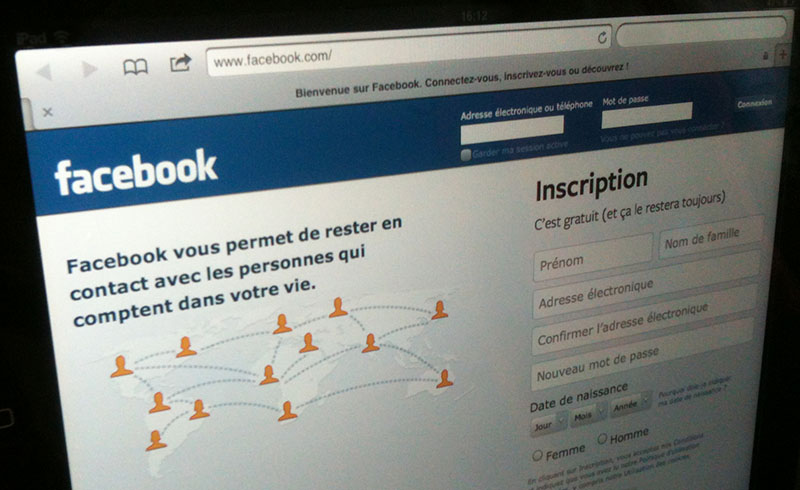
\includegraphics[width=\linewidth]{graphII-01-facebook.jpg}
\end{graphic}
\vspace{-\baselineskip}

\textsc{Facebook} connecte près d'un milliard de personnes. Chacune d'elles a un profil personnel, un compte qui comprend notamment un journal --- précédemment appelé « mur » --- sur lequel elle publie des informations la concernant et un fil d'actualité duquel elle voit défiler les activités de ses « amis » : leurs photos, les articles qu'ils partagent, leurs commentaires sur des articles postés par d'autres, etc.

Chaque utilisateur de \textsc{Facebook} ayant en moyenne plusieurs centaines d'amis, tous les éléments que ceux-ci postent sur la plateforme, communément appelés \textit{posts}, n'apparaissent pas dans son fil d'actualité, loin s'en faut. \textsc{Facebook} opère en réalité une sélection radicale. D'une part, pour ne pas inonder les comptes d'informations qui disparaîtraient en une fraction de seconde à cause de leur trop grand nombre. D'autre part, pour faire en sorte que chaque personne trouve son fil d'actualité suffisamment intéressant pour rester connectée et active sur son compte. Car plus il y a de personnes connectées et plus \textsc{Facebook} peut monnayer son support publicitaire.

Mais sur quoi \textsc{Facebook} se fonde-t-il pour faire sa sélection ?

Pour décider ce qui va être affiché dans un fil d'actualité, \textsc{Facebook} utilise un algorithme parfois appelé \textit{Edge Rank}. Son principe de fonctionnement n'a rien de sorcier. 

Pour chaque utilisateur « U », \textsc{Facebook} calcule le score des informations (photo, note, article, commentaire, etc.) postées par ses amis. Le score d'un post « p » publié par l'un de ses amis « X », que l'on peut noter ici par » $score(p)$ », correspond \textit{grosso modo} au produit de trois variables, à savoir :
\begin{equation}
%\begin{array}{@{}c@{}}
score(p) = A × T × F\\
%\mbox{où } \left\{
%\begin{tabular}[c]{@{\,}p{0.75\linewidth}@{}}
%A désigne l'affinité de U par rapport à X : plus U a l'habitude de commenter des informations postées par X, plus A sera grand. \\[-1.5pt]
%T dépend du type de l'élément posté : ainsi, T sera plus élevé pour un élément de type photo que pour un petit texte par exemple. \\[-1.5pt]
%F représente la fraîcheur du post : plus un post est ancien, plus F diminue.
%\end{tabular} \right.
%\end{array}
\end{equation}

\begin{itemize}
\item A désigne l'affinité de U par rapport à X : plus U a l'habitude de commenter des informations postées par X, plus A sera grand.
\item T dépend du type de l'élément posté : ainsi, T sera plus élevé pour un élément de type photo que pour un petit texte par exemple.
\item F représente la fraîcheur du \textit{post} : plus un \textit{post} est ancien, plus F diminue.
\end{itemize}

\textsc{Facebook} calcule périodiquement les scores de toutes les informations postées par les amis de U et affiche dans le fil d'actualité de U celles qui ont le score le plus élevé.

\begin{marginvideo}
	[\label{vid:II.3}Algorithme \emph{Redge rank}, fil d'actualité \textsc{Facebook}.]%
	\href{https://www.youtube.com/watch?v=1ParbwnSJpM}%
		{
\includegraphics[width=\marginparwidth]{./Images/Pictograms/film-strip-dark-electric-blue.png}}%
	%\movie[width=\marginparwidth,showcontrols]%
	%	{
\includegraphics[width=\marginparwidth]{./Images/Pictograms/film-strip-dark-electric-blue.png}}%
	%	{./Videos/Chapter02/vidII-01-algorithme-edge-rank-facebook-Rachid-Guerraoui.mp4}%
	\launchvideo{https://www.youtube.com/watch?v=1ParbwnSJpM}
\end{marginvideo}

Précédemment, il a été indiqué qu'approximativement le score correspond au produit des trois variables. En fait, il s’agit plus précisément d’une somme de produits, car chaque information peut avoir été commentée par plusieurs utilisateurs, et chaque commentaire contribue à augmenter son score.

Pour une explication plus complète du principe de l’algorithme \textit{Edge Rank} de \textsc{Facebook}, visionner la \cref{vid:II.3} (durée : 10 min).


\begin{gofurther}
\begin{itemize}\jazzitem
\item \href{https://pixees.fr/autour-du-web/}{Autour du Web}, Fabien \textsc{Gandon}, \textsc{Pixees} ;
\item \href{https://pixees.fr/les-quatre-facettes-du-web/}{Les quatre facettes du Web}, Fabien \textsc{Gandon}, \textsc{Pixees} ;
\item \href{https://fr.slideshare.net/fabien_gandon/web-smantique-et-web-social-1700977}{Web sémantique et Web social}, Fabien \textsc{Gandon}, 2009 ;
\item Caractéristiques communes aux services de réseaux sociaux, CBPL Commission de la protection de la vie privée ;
\item \href{http://ses.ens-lyon.fr/articles/les-reseaux-sociaux-138014}{Les réseaux sociaux}, une vision par le sociologue Pierre \textsc{Mercklé}. SES-ENS,  11/03/2012 ;
\item \href{https://www.internetsanscrainte.fr/programmes/vinz-et-lou}{2025 Exmachina}, Internet sans crainte, jeu sérieux d'éducation critique à Internet. Une production Tralalère avec la participation du CNC, le soutien de la Commission européenne et de la Délégation aux Usages de l’Internet dans le cadre d’Internet Sans Crainte ;
\item \href{http://www.mshsud.tv/spip.php?article214}{L’internet social (ou Web 2.0) : opportunités, impact et défi}, Patrick \textsc{Valduriez}, MSH-M TV,  9 février 2010 ;
\item \href{https://www.youtube.com/watch?v=jNjHdqS-1Ko}{Les (r)évolutions de la planète Web}, Agora Des Savoirs 2015 ;
\item \href{https://www.canal-u.tv/video/inria/les_algorithmes_de_classement_utilises_dans_les_moteurs_de_recherche.6608}{Les algorithmes de classement utilisés dans les moteurs de recherche}, Conférence de Michel \textsc{Habib}, \textsc{Canal U}, collection \textsc{Inria} Science Info Lycée Profs, 63 mn, Juin 2009.  Comment fonctionne \textsc{Google}.
\end{itemize}
\end{gofurther}


%----------
\section[Calcul dans les nuages]{Calcul dans les nuages : \textit{Cloud Computing}}
\label{sec:II.2}

La plupart des gens ont déjà entendu parler du « \gls{cloud} ».\caution[t]<secondcolor>{%
Spécialiste des données, de l’information et des connaissances, la recherche de \href{https://fr.wikipedia.org/wiki/Serge_Abiteboul}{Serge \textsc{Abiteboul}} porte notamment sur la gestion d'informations sur le Web et la gestion de données personnelles. Ces sujets sont aujourd'hui essentiels face à l'accroissement et à la « massification » des données.\\
Directeur de recherche \textsc{Inria} et professeur affilié à l’École normale supérieure de Cachan, Serge \textsc{Abiteboul} est diplômé de Télécom-Paris, a obtenu un Ph.D. de l'\textit{University of Southern California} et une Thèse d'État de l'Université \textsc{Paris-Sud}. Il est membre de l'Académie des Sciences et de l'Académie Europae, du Conseil scientifique de la SIF.
Il a occupé la \href{http://www.college-de-france.fr/site/serge-abiteboul/}{Chaire d'informatique au Collège de France} (2011-2012) et la \href{https://www.info.fundp.ac.be/francqui2013/}{Chaire Francqui à l'Université de Namur} (2012-2013). Il a été membre du \href{https://cnnumerique.fr/}{Conseil national du numérique} (2013-2016).\\
Il anime avec des amis le blog invité du Monde.fr, \url{binaire.blog.lemonde.fr}, dont il est le fondateur.}{À propos de l'intervenant} Pourtant, peu de personnes savent exactement de quoi il retourne...

%\vspace*{-0.5pt}
\subsection[Quid du \textit{cloud} ?]{Quid du \textit{cloud} ?}
\label{sub:II.2.1}

\subsubsection[Infrastructure]{Infrastructure}
\label{subsub:II.2.1.1}

\paragraph*{Définition} Pour définir le « \textit{cloud} » --- nuage en anglais ---, il faut peut-être revenir à ce qu'est l'informatique, soit d'une part, des données et d'autre part, des calculs effectués par des processeurs. 

Chacun a l'habitude de son ordinateur personnel constitué de mémoires, d'un disque dur et d'un processeur. Cet ensemble calcule à domicile. Le concept de « \textit{cloud} » est de déporter cette capacité de calcul hors de chez soi, dans « les nuages », c'est-à-dire probablement dans un \gls{datacenter} --- ou centre de données en français ---, qui peut parfois se situer de l'autre coté de la planète.

Le terme de \textit{cloud} provient de la représentation d'Internet sous forme de nuage. À partir du moment où on va déposer ses calculs et ses données sur Internet, on va les mettre dans les nuages. Par extension, on va alors parler de calcul dans les nuages : \textit{cloud computing}.

En fait, il ne s'agit pas de quelque chose « d'évaporé », ce sont des éléments bien physiques ; des ordinateurs et des disques qui ne résident pas au domicile de l'utilisateur, mais quelque part dans le monde... Dont on ne connaît même pas la localisation.

\begin{marginvideo}
	[\label{vid:II.4}\textup{Cloud computing}.]%
	\href{https://www.youtube.com/watch?v=5YawCCUxa_E&list=PLWvGMqXvyJAMNWRvODUB5Ry3licACdaa0&index=13}%
		{
\includegraphics[width=\marginparwidth]{./Images/Pictograms/film-strip-dark-electric-blue.png}}%
	%\movie[width=\marginparwidth,showcontrols]%
	%	{
\includegraphics[width=\marginparwidth]{./Images/Pictograms/film-strip-dark-electric-blue.png}}%
	%	{./Videos/Chapter02/vidII-02-cloud-HD.mp4}%
	\launchvideo{https://www.youtube.com/watch?v=5YawCCUxa_E&list=PLWvGMqXvyJAMNWRvODUB5Ry3licACdaa0&index=13}
\end{marginvideo}

\paragraph*{Aspects technologiques} Pour bien comprendre le \textit{cloud}, il faut correctement appréhender ce qui a permis sa réalisation. 

À l'origine de la création du \textit{cloud}, il y a d'abord et principalement des réseaux hyper rapides qui connectent une entreprise ou la maison d'un particulier aux centres de données.

Par ailleurs, la seconde raison est liée à la baisse considérable des coûts des machines, des disques et du stockage qui sont devenus quasiment marginaux. 

À partir de là, cela devient possible de concentrer dans un même lieu quantité de processeurs et de moyens de stockage puis de déporter l'ensemble de cette infrastructure.

La difficulté technique est de faire fonctionner ces gigantesques entrepôts de données. Deux problèmes majeurs se posent :
\begin{enumerate}
\item \emph{la dissipation de la chaleur} --- La concentration des ordinateurs génère une chaleur considérable qui demande de climatiser en permanence le \textit{data center}. Des progrès remarquables en climatisation ont ainsi été réalisés ;
\item \emph{la gestion des pannes} --- Statistiquement, un ordinateur va au bout d'un certain temps avoir une panne matérielle ou logicielle. Quand un million de processeurs sont placés dans un même entrepôt, la probabilité d'une panne devient très importante. Il faut donc avoir les moyens techniques de pallier cette problématique. Lorsqu'une panne se produit sur une application, on ne s'en aperçoit pas forcément car un autre ordinateur va automatiquement prendre le relais pour continuer son exécution. Beaucoup d'algorithmes ont été développés en ce sens.
\end{enumerate}


\subsubsection[Problématique]{Problématique des contraires}% positives et négatives
\label{subsub:II.2.1.3}


\paragraph*{Atouts et avantages} Lorsque des données sont placées dans le \textit{cloud}, la première garantie est celle de la \gls{cloudsafety}. Ces informations ne disparaîtront pas car elles sont probablement répliquées en plusieurs endroits, voire plusieurs centres de données.

Cette protection des données est également valable contre les intrusions. Ce n'est pas assuré à 100\% mais, les compétences des personnels des \textit{data center} sont certainement supérieures à celle d'un particulier ou d'une entreprise dont le métier n'est pas l'informatique.

Justement, un deuxième avantage du \textit{cloud} pour les entreprises est de réaliser des économies de gestion. Ce n'est pas le cœur de métier, par exemple d'une entreprise de travaux publics, d'acheter et de gérer un parc informatique, ni d'embaucher et d'encadrer des \gls{system-engineer} et réseaux. Ainsi, le \textit{cloud} permet d'\gls{externalizing} ces services en perdant un peu le contrôle sur ses données.

\paragraph*{Inconvénients et améliorations} Beaucoup de points positifs du \textit{cloud} ont jusqu'à présent été soulignés. Il existe néanmoins quelques aspects négatifs qui sont à exposer.

Tout d'abord les questions écologiques sont à préciser. En effet, quand les données sont distantes de plusieurs milliers de kilomètres cela génère une consommation d'énergie importante, voire des gaspillage, pour les rapatrier.

Un second point concerne un aspect sous-jacent relatif à  une hyper-centralisation des calculs et des données. À l'arrivée, seules quelques entreprises \pagebreak possèdent toutes les données personnelles des individus dans d'énormes centres de données. C'est un constat qui s'oppose à la philosophie originelle de l'Internet qui est plutôt de décentraliser et localiser les données et leur traitement. La décentralisation a beaucoup d'avantages ; elle rend plus autonome et mène entre autres à des économies d'énergie.

Pour améliorer les choses, on pourrait justement imaginer de déconcentrer les \textit{data center}. L'ensemble des équipements domestiques, de la télévision au téléphone mobile, sont des ordinateurs. Ce sont ce type d'ordinateurs qui pourraient localement conduire des calculs dans les nuages. En prenant l'exemple de la vidéo, plutôt que d'aller chercher un programme à l'autre bout du monde et dépenser inutilement de l'énergie, il serait possible de récupérer ce contenu au niveau régional ou local chez un voisin, lequel ne s’apercevrait même pas qu'il va servir un film. Ainsi, des économie substancielles d'énergie pourraient se réaliser, de même que retrouver l'esprit originel de décentralisation de l'Internet et du Web.

\printlocalglossary{8}


\subsection[\textit{Cozy Cloud} : nécessaire vertu]{\textit{Cozy Cloud} : vertueux par nécessité}
\label{sub:II.2.2}

\begingroup\itshape
Serge Abiteboul nous parle d’une \textup{startup}, \textsc{Cozy Cloud},\caution[t]<firstcolor>{%
\upshape Texte rédigé par Serge \textsc{Abiteboul} et publié sur \href{https://www.lemonde.fr/blog/binaire/2016/02/04/cozy-cloud-vertueux-par-necessite/}{Binaire} --- blog du numérique du journal \textsc{Le Monde} --- le 4 février 2016.}{\upshape Note de la rédaction}
 qui développe un système de gestion d’informations personnelles. Il nous explique ce que sont ses systèmes, quels sont leurs buts. Avec les enjeux autour du contrôle des données personnelles, cette nouvelle approche prend tout son sens. Une \textup{startup} qui mérite vraiment qu’on la suive de près.
\endgroup

\begin{tcolorbox}[boxrule=0pt, arc=0pt, boxsep=0pt, top=4pt, bottom=4pt, left=4pt, right=4pt]
2 février 2016 --- La \textit{startup} \textsc{Cozy Cloud} et le bureau d’enregistrement \textsc{Gandi} sont lauréats de la 2\frup{ième} édition du Concours d’innovation numérique pour leur projet de \textit{cloud} personnel grand public.
\end{tcolorbox}

Nos données sont un peu partout, dans des services, dans de plus en plus de services différents. Nous finissons par ne plus très bien savoir où elles sont, ni même ce qu’elles sont ou ce qu’on fait avec. Donc, nous ne nous y retrouvons plus. Par exemple, nous nous rappelons que nous avons l’adresse de ce copain, mais nous ne savons pas la trouver : dans nos contacts, dans nos mails, sur \textsc{LinkedIn}, sur \textsc{Facebook}, dans un SMS peut-être ou qui sait, sur \textsc{WhatsApp}... Chacun de ces systèmes nous rend un service particulier, mais leur multiplication devient chaque jour un peu plus notre problème. Des systèmes se proposent de corriger cela, les systèmes de gestion de données personnelles, les \emph{Pims} pour \textit{Personal Information Management Systems}.

\sidequote[Benjamin \textsc{André}, \textsc{Pdg}  \href{https://cozy.io/fr/}{\textsc{Cozy Cloud}}]{Si vos données sont partout, c’est qu’elles ne sont nulle part.}%
L’idée est simple : plutôt que de regrouper les données par services (les données sur les courriels de millions d’utilisateurs avec \textsc{Gmail}, sur les films avec \textsc{Netflix}, sur les déplacements avec \textsc{Waze}, etc.), on va regrouper les données par utilisateur. Donc nous aurons notre système à nous, pour nous, avec toutes les données des applications que nous utilisons. Ces données, nous voudrions qu’elles soient disponibles en permanence, de partout, on va dire que c’est « notre \textit{cloud} personnel~».

\sidegraphic{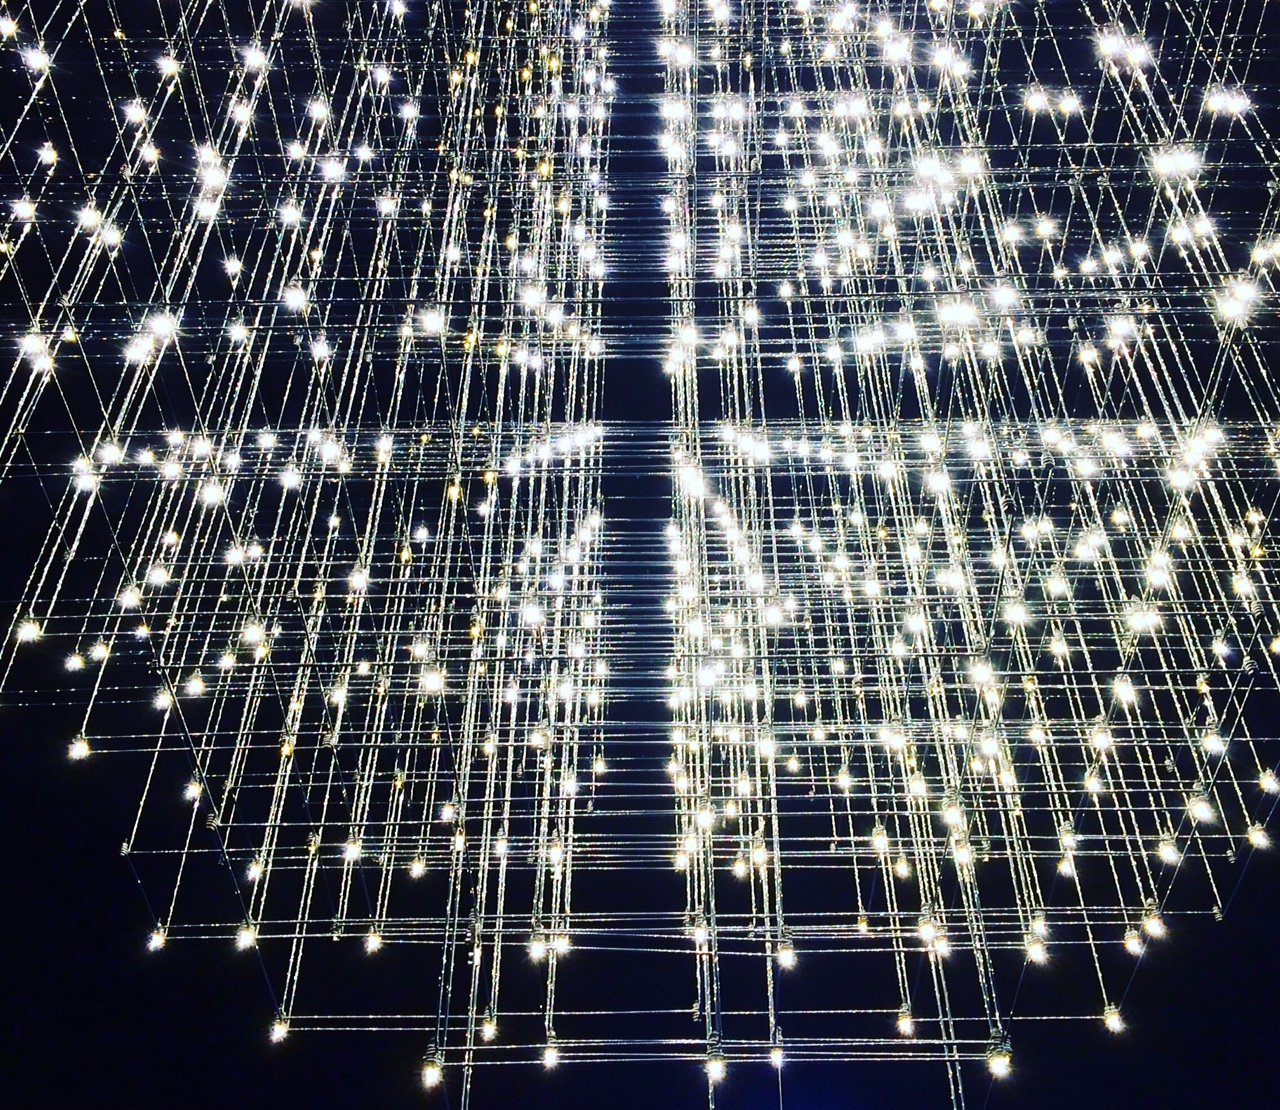
\includegraphics[width=\linewidth]{graphII-02-binaire-abiteboul-maev59.jpg}}{@maev59}
Pourquoi promouvoir les \textit{Pims} ? Parce que la situation actuelle avec quelques sociétés --- en caricaturant, les géants du Web ---, qui s’approprient toutes les données du monde est fondamentalement malsaine. D’abord, à terme, nous y perdons notre liberté : nous sommes profilés par ceux qui savent tout de nous, qui choisissent pour nous ; et les services qu’ils nous offrent deviennent incontournables parce qu'eux seuls ont certaines informations et peuvent les fournir. Ensuite, ces grandes sociétés finissent par être à même d’étouffer la compétition. Internet et le Web qui ont servi véritablement de catalyse pour l’innovation, sont en train de devenir le royaume des oligopoles, les fossoyeurs des belles idées de liberté et de diffusion libre des connaissances des débuts. Bon, c’est un résumé un peu rapide, un peu brutal. Mais le lecteur intéressé pourra trouver un développement de ces idées \parencite{Abiteboul-et-al:2015} dans CACM, la principale revue de l’ACM, une organisation internationale dédiée à l’informatique.

Donc, partons de l’hypothèse qu’il faille que chacun regroupe toutes ses données dans un système unique. Un \textit{geek} saura installer un serveur et, en voiture \textsc{Linux} ! Mais la plupart des gens n’ont pas cette compétence et, même s’ils l’ont ou pourraient l’acquérir, ils ont probablement d’autres façons de dépenser leurs temps libre : le sport, les expos, le farniente...

Il y aurait bien une solution, ce serait de choisir les grands de l’Internet. Pourquoi pas tout mettre chez eux ? Parce que nous aimerions avoir confiance dans le gardien de nos données. La confiance, le gros mot... Nous avons fait confiance aux fondateurs de \textsc{Google}, \textsc{Brin} et \textsc{Page}, quand ils disaient « \textit{Don’t be evil !} ». Mais qui dirige \textsc{Google} aujourd’hui ? Des actionnaires qui veulent maximiser leurs revenus ? Pour protéger nos données personnelles, nous aimerions plus que de vagues promesses. Nous voulons des garanties ! Nous allons donc plutôt choisir un tiers de confiance.

\sidegraphic[Copie d'écran : bureau de Cozy Cloud]{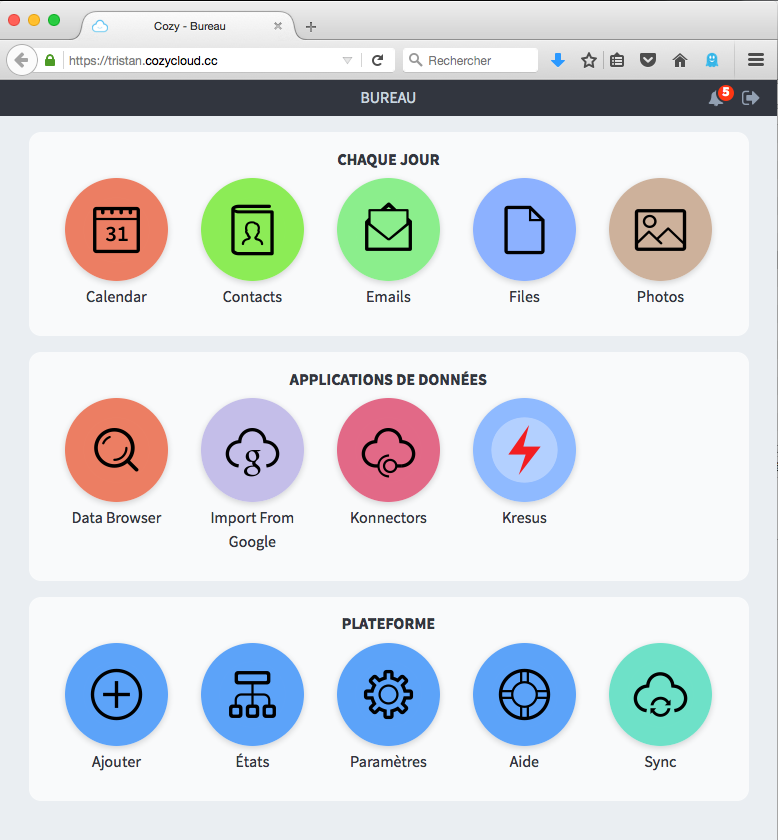
\includegraphics[width=\linewidth]{graphII-03-bureau-cozy.png}}
Un de ces tiers de confiance possibles, c’est la \textit{startup} \textsc{Cozy Cloud}. Pour écrire cet article, j’ai rencontré son \textsc{Pdg} Benjamin \textsc{André}. J’ai aussi côtoyé au Conseil national du numérique, son CPO --- \textit{Chief Product Officer} ---, Tristan \textsc{Nitot}. Je suis fan des deux. Il faut rajouter que je suis un fervent supporteur des \textit{Pims} et que ma recherche porte sur les \textit{Pims}. Donc je ne suis pas toujours objectif quand j’en parle. Je pourrais parler objectivement de la recherche sur des \textit{Pims}. Mais ce n’est pas le sujet de cet article. Ce qui m’intéresse ici c’est la gestion de données avec des \textit{Pims} comme levier pour aller vers une société meilleure. Donc j’ai plus une casquette de militant que de scientifique. Cet article ne revendique donc aucune objectivité. Pourtant, je tiens quand même à souligner pour éviter les malentendus que je n’ai aucune participation financière dans \textsc{Cozy Cloud} ou d’ailleurs toute autre société de \textit{Pims}.

Un vrai argument des \textit{Pims} (en tous cas, dans ma vision), c’est que leur logiciel est \textit{open-source}. Bien sûr, nous n’avons pas le temps d’aller auditer leur code, mais d’autres peuvent le faire pour nous. Cette transparence sur la gestion des données est essentielle pour garantir que la plateforme ne va pas faire n’importe quoi avec nos données. Excusez du peu. Sans vouloir nous angoisser, toutes les données que nous avons à droite ou à gauche, des informations peut-être stratégiques pour nos entreprises, des informations intimes sûrement, les nôtres et celles de nos amis. Nous ne savons pas ce qu’on fait d’elles. Nous ne savons pas où elles atterrissent. Bon le mieux, c’est de ne pas trop y penser, ça va pourrir l’ambiance.

\sidequote[Tristan \textsc{Nitot}, \textsc{CPO}  \href{https://cozy.io/fr/}{\textsc{Cozy Cloud}}\\ \footnotesize\textcolor{firstcolor}{\faTwitter} : @nitot]{La portabilité des données, c’est\\ la possibilité pour un internaute\\ de récupérer ses données depuis\\ les grands services centralisés\\ pour les mettre où il le veut.\\ Pour lui, c’est une liberté\\ fondamentale, celle de pouvoir\\ « déplacer sa vie numérique » où\\ bon lui semble, y compris chez lui.}%
Le fait que le logiciel de la plate-forme soit en \textit{open-source} et donc la transparence qui en résulte, est une qualité essentielle de ces systèmes. Cela facilite la vérification. Il faut aussi mentionner un autre aspect : la « portabilité ». N’ayez pas peur, c’est technique mais cela s’explique très bien.

Pour comprendre la portabilité, prenons un exemple de portabilité dans un autre domaine, l’automobile. Nous avons une \textsc{Peugeot}. Et puis, un jour, nous voulons changer de voiture. Nous sommes libres, d’acheter une \textsc{Renault}, même une \textsc{Volkswagen}, ce que nous voulons. Notre expérience de conducteur, nous la « portons » sous d’autres cieux. Nous n’avons pas à réapprendre. Dans les applications numériques, ça peut être différent. Nous avons choisi le \textsc{Kindle} d’\textsc{Amazon}. Et bien, c’est un super système, mais nous nous sommes fait avoir. Nous ne pouvons pas passer à un autre système sans perdre toute la librairie que nous avons achetée. Nous accumulons des années d’information, de données, dans un système et on nous dit « Restes avec nous ou perds tout !~» C’est l’emprisonnement par le vendeur, « \textit{vendor lock-in} » en anglais. Nous aimerions pouvoir partir en « emportant » nos données dans le nouveau système --- sans avoir à payer en argent, en temps, en quoi que ce soit. Le système doit nous garantir la portabilité, c’est-à-dire votre liberté de dire quand nous le souhaitons : « Ciao ! Sans rancune~».

\sidegraphic{
\includegraphics[width=0.75\linewidth]{cozycloud-logo.pdf}}
Des systèmes comme \textsc{Cozy Cloud} nous permettent de partir quand nous le voulons, avec nos données. Nous restons si nous le voulons. C’est drôle de réaliser que le droit de partir peut devenir un argument pour choisir de rester. \textsc{Google} disait « \textit{Don’t be evil} » et il fallait croire sur parole qu’ils ne seront pas diaboliques. Dans un système qui garantit structurellement la portabilité, nous n’avons pas à les croire, ils n’ont d’autre choix que d’être angéliques s’ils veulent que nous restions. Cela pourrait être indiqué dans la loi. Des gens y travaillent.

\begin{tcolorbox}[boxrule=0pt, arc=0pt, boxsep=0pt, top=4pt, bottom=4pt, left=4pt, right=4pt]
Les députés ont validé le principe de récupération des données personnelles par les internautes. Il sera ainsi possible de transférer sa playlist \textsc{iTunes} vers \textsc{Spotify} ou ses photos \textsc{Instagram} vers une autre application. En revanche, cette obligation ne s’appliquerait qu’aux services grand public, excluant, devant la levée de boucliers des éditeurs de logiciels, les services inter-entreprises. Le Monde Économie, Sarah Belouezzane et Sandrine Cassini, 19 janvier 2016. 
\end{tcolorbox}

Essayons de comprendre un peu mieux la techno. \textsc{Cozy Cloud} développe une plateforme pour gérer nos données personnelles. Nous pourrons un jour tout y mettre, nos contacts, nos courriels, nos déplacements GPS, nos documents, nos comptes bancaires, notre compta... Ils nous proposent des applications qui réalisent certaines fonctionnalités (comme l’agenda) ou qui nous permettent juste de récupérer nos données d’autres services, par exemple nos mails de \textsc{Gmail}. Cette plateforme, nous pouvons l’installer sur une machine personnelle, ou nous pouvons demander à une société de l’héberger pour nous, par exemple OVH. Et à quoi sert \textsc{Cozy Cloud} à part développer la plate-forme ? Ils peuvent gérer le système pour nous.

Nous n’avons pas dit grand-chose du \textit{business model} de \textsc{Cozy Cloud}. Bien sûr, c’est une \textit{startup}, alors ils ont un \textit{business model} qui montre qu’ils veulent se développer, ils cherchent des investisseurs, ils vont gagner plein d’argent. Mais nous pensons --- nous espérons sans nous tromper --- que Benjamin \textsc{André}, Tristan \textsc{Nitot} et les autres de \textsc{Cozy Cloud} veulent d’abord changer le monde, en faire un endroit où il fait meilleur de vivre. Nous avons l’impression d’avoir entendu ça des tas de fois ; ça peut prêter un peu à sourire ; mais avec \textsc{Cozy Cloud}, c’est tellement rafraîchissant.

Allez, un peu de fiction pour conclure, tout en restant conscient de la difficulté de prédire l’avenir. Nous aurons (bientôt) toutes nos données chez l’hébergeur de notre choix, elles seront gérées par un \textit{cloud} personnel fonctionnant avec \textsc{Cozy Cloud} (\textit{Pimseur} français) qui procurera un point d’entrée unique à toutes nos données. Le système les rendra accessibles de partout, les synchronisera, les archivera, gérera nos Internet des objets, servira d’assistant personnel, suivra notre santé, notre vie sociale. Nous pourrons réaliser des analyses qui utilisent nos données mais qui, contrairement aux analyses \textit{Big data} des autres, le fera pour notre bien et non pour maximiser le profit des autres. Et puis notre \textit{Pims} pourra causer avec les \textit{Pims} de nos amis...  C’est dingue, nous étions totalement périphériques dans le monde des \textsc{Gafas}, nous voilà transportés au centre du monde grâce aux \textit{Pims}...

\begin{gofurther}
\begin{itemize}\jazzitem
\item \href{https://www.lemonde.fr/blog/binaire/2016/05/30/les-donnees-dans-les-nuages/}{Les données dans les nuages}, Serge \textsc{Abiteboul}, Benjamin \textsc{Nguyen} et Philippe \textsc{Rigaux}, \textsc{Binaire}, 30 mai 2016 ;
\item \href{https://interstices.info/calculer-dans-les-nuages/}{Calculer dans les nuages}, Patrick \textsc{Valduriez} et Joanna \textsc{Jongwane}, \textsc{Interstices}, 2011 (\textit{podcast} 12 mn) ;
\item \href{https://dl.acm.org/doi/pdf/10.1145/2670528?download=true}{\textit{Managing your digital life}}, Serge \textsc{Abiteboul}, Benjamin \textsc{André} et Daniel \textsc{Kaplan}, Communications of the ACM, 58:5, 2015 ;
\end{itemize}
\end{gofurther}


%----------
\section[Monnaies cryptographiques]{Monnaies cryptographiques}
\label{sec:II.3}



%\vspace*{-0.5pt}
\subsection[Du \textit{bitcoin} à la \textit{blockchain}]{Du \textit{bitcoin} à la \textit{blockchain}}
\label{sub:II.3.1}

Le \gls{bitcoin} est une monnaie planétaire,\caution[t]<secondcolor>{%
Informaticien et mathématicien, \href{http://www.lifl.fr/~jdelahay/}{Jean-Paul \textsc{Delahaye}} est professeur émérite à l'Université de Lille et chercheur au \href{https://www.cristal.univ-lille.fr/}{CRISTAL} (Centre de recherche en informatique, signal et automatique de Lille, UMR CNRS 9189).\\
Spécialiste en théorie de la complexité, il mène aussi des travaux dans le domaine de la modélisation et s'intéresse à l'utilisation et à la définition du hasard en informatique.\\
Jean-Paul \textsc{Delahaye} a publié de nombreux ouvrages scientifiques destinés à un large public. Il a reçu le Prix \textsc{d'Alembert} 1998 de la Société Mathématique de France pour « \textit{Le Fascinant nombre Pi} » et le Premier prix Auteur 1999 de la\linebreak Culture scientifique du Ministère de l'é\-ducation nationale, de la recherche et de la technologie.}{À propos de l'intervenant}
 \href{https://fr.wikipedia.org/wiki/Cryptomonnaie}{cryptographique}, fondée sur un système de transaction et de contrôle \href{https://fr.wikipedia.org/wiki/Pair_%C3%A0_pair}{peer-to-peer} --- pair à pair en français ---, la \href{https://fr.wikipedia.org/wiki/Blockchain}{\textit{blockchain}} --- littéralement « chaîne de blocs ». Comment cela fonctionne-t-il ? Quels en sont les enjeux ? Quels liens avec la  sécurité de nos données, ici nos transactions bancaires ? C'est une véritable « révolution numérique ».

\subsubsection[Monnaie numérique]{Monnaie numérique}
\label{subsub:II.3.1.1}

L'argent peut-il exister sous forme numérique ? C'est une question à laquelle on peut répondre de plusieurs manières.

Déjà, chacun sait que lorsqu’on utilise une carte bancaire ou réalise un virement par Internet, c'est de l'argent numérique en fin de compte qui circule. Cependant, il existe depuis 2009 une autre forme de monnaie numérique plus intéressante qui, au niveau du développement de l'informatique et des idées va sans doute avoir un grand rôle ; c'est ce que l'on nomme sous le terme de monnaies cryptographiques, dont le \textit{bitcoin} est le premier exemple.

\overparagraph{Fonctionnement}

\begin{marginvideo}
	[\label{vid:II.5}Monnaies cryptographiques.]%
	\href{https://www.youtube.com/watch?v=a3EHogSreCs&list=PLWvGMqXvyJAMNWRvODUB5Ry3licACdaa0&index=14}%
		{
\includegraphics[width=\marginparwidth]{./Images/Pictograms/film-strip-dark-electric-blue.png}}%
	%\movie[width=\marginparwidth,showcontrols]%
	%	{
\includegraphics[width=\marginparwidth]{./Images/Pictograms/film-strip-dark-electric-blue.png}}%
	%	{./Videos/Chapter02/vidII-03-money-full.mp4}%
	\launchvideo{https://www.youtube.com/watch?v=a3EHogSreCs&list=PLWvGMqXvyJAMNWRvODUB5Ry3licACdaa0&index=14}
	%\includemedia[
  %width=\linewidth,
  %%totalheight=0.225\linewidth,
  %activate=pageopen,
  %passcontext,  %show VPlayer's right-click menu
  %addresource=./Videos/Chapter02/vidII-03-money-full.mp4,
  %flashvars={
  %  %important: same path as in `addresource'
  %  source=./Videos/Chapter02/vidII-03-money-full.mp4
  %}
	%]{
\includegraphics[width=\marginparwidth]{./Images/Pictograms/film-strip-dark-electric-blue.png}}{VPlayer.swf}
\end{marginvideo}

Le \textit{bitcoin} est une monnaie créée \textit{ex-nihilo} le 3 janvier 2009 en utilisant un réseau pair à pair. Son ou ses auteurs sont connus sous le pseudonyme de Satoshi \textsc{Nakamoto}, mais personne ne sait à qui il renvoie. Cette personne ou ce groupe a décrit le protocole, s'est arrangé pour écrire les programmes qui le font fonctionner et l'a mis en œuvre. 

Ce protocole a aujourd'hui généré une monnaie qui s'appelle le \textit{bitcoin}, dont la capitalisation totale vaut actuellement 10 milliards d'euros ; ce qui est tout de même considérable. 

Donc le bitcoin est une monnaie réelle, qui n'existe que sous forme numérique, il n'y a pas de billets, il n'y a pas de pièces bitcoin, c'est quelque chose qui circule uniquement sur les réseaux et dont le fonctionnement est fondé sur ce qu'on appelle un \emph{fichier partagé} --- on dit aussi un \emph{registre partagé} --- qu'on appelle la \emph{blockchain}.

Pour comprendre le fonctionnement du \textit{bitcoin}, il faut saisir le con\-cept de \textit{blockchain}. L'idée en elle-même est assez simple. Elle peut se formuler comme suit : « \textit{si tout le monde est d'accord pour savoir qui possède des \textup{bitcoins}, ceux-ci n'ont pas besoin d'être réels, c'est-à-dire matérialisés par des pièces métalliques, en or, en argent ou de quelconque nature}~».

Cela semble un petit peu bizarre et, au début, on a du mal à y croire, mais cela fonctionne. Il existe ainsi un fichier\sidenote{Techniquement, il s'agit d'une base de données distribuée, vérifiée par blocs et sécurisée par cryptographie (source \href{https://fr.wikipedia.org/wiki/Blockchain}{\faWikipediaW}).} qui s'appelle 
la \textit{blockchain}, qui indique précisément ce que détient chaque compte. Par le fait que ce fichier soit reproduit en de multiples exemplaires sur des ordinateurs différents --- à peu près 5\,000 dans le cas du \textit{bitcoin} ---, cela crée une sorte de confiance entre les utilisateurs car personne ne peut tricher en modifiant à sa guise le contenu du fichier, personne ne peut créer de \textit{bitcoins} nouveaux sans que ce soit prévu par le fonctionnement général. L'origine de cette confiance est fournie par le partage de l'information. Le principe de la \textit{blockchain} peut se généraliser à bien d'autres fonctions qu'un système monétaire.

\begin{marginfigure}%
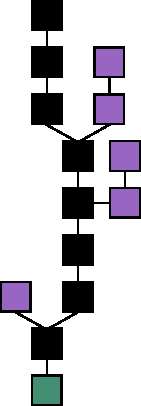
\includegraphics[width=0.5\linewidth]{figII-03-blockchain.pdf}
\caption{\label{fig:II.3}Représentation d’une chaî\-ne de blocs. La chaîne principale (noir) est composée de la plus longue suite de blocs après le bloc initial (vert). Les blocs orphelins sont violet (d'après \href{https://fr.wikipedia.org/wiki/Blockchain}{\normalfont\faWikipediaW}).}
\end{marginfigure}


\overparagraph{Fiabilité}

Les \textit{blockchains}, en particulier celle du \textit{bitcoin}, se fondent sur les primitives de ce qu'on appelle la cryptographie mathématique. Ce sont elles qui créent la solidité des informations qui sont gérées par la \textit{blockchain}. Il en est de même de la fiabilité et de l'indestructibilité de ces informations. Tous les développements dérivés du \textit{bitcoin} et de la \textit{blockchain} sont issus des mathématiques, c'est une chose assez remarquable pour être soulignée. 

C'est ainsi la maîtrise que l'on a aujourd'hui des protocoles de cryptographie, en particulier des systèmes de signatures numériques, des systèmes de hachage de fichiers, qui permet au protocole de fonctionner sans que personne ne puisse tricher. Car le cœur de la problématique est là, il ne faut pas que quelqu'un puisse manipuler le protocole pour s'attribuer de l'argent ou autre chose quand il s'agit d'une autre \textit{blockchain}. Donc les mathématiques, et spécifiquement la cryptographie mathématique, grâce à la maturité de cette science informatique et numérique, sont à la base du \textit{bitcoin} et de la \textit{blockchain}.  

\overparagraph{Transactions}

Dans le protocole du \textit{bitcoin}, il existe\sidenote{Le principe est équivalent pour d'autres \textit{blockchains}.} des signatures numériques ou cryptographiques. Quand quelqu'un détient des \textit{bitcoins}, il dispose de deux informations. La première est son numéro de compte, comme un numéro de compte bancaire, que l'on va appeler la \emph{clé publique}. La seconde est une \emph{clef secrète}. Lors d'une transaction, le détenteur du compte va pouvoir la signer en utilisant sa clef privée au travers du réseau. Lui seul peut signer une transaction puisque lui seul possède cette clé privée. Dans le même temps, tous ceux qui 
connaissent son numéro de compte vont pouvoir vérifier que c'est bien lui qui a signé. C'est un petit miracle mathématique offert par les cryptologues : ces systèmes à double clefs permettent à tout le monde de vérifier qu'une signature est bonne.

\sidegraphic{
\includegraphics[width=.75\linewidth]{bitcoin-logo.pdf}}%
Cette procédure est évidemment essentielle dans le protocole \textit{bitcoin} ; il ne s'agit pas simplement que certains comptes détiennent de l'argent, il faut aussi qu'il puisse circuler. Néanmoins, seul le détenteur d'un compte peut établir une transaction vers un autre.

\subsubsection[Impacts]{Impacts}
\label{subsub:II.3.1.2}


\overparagraph{Extensions cryptographiques}

\sidegraphic[Diverses monnaies cryptographiques.]{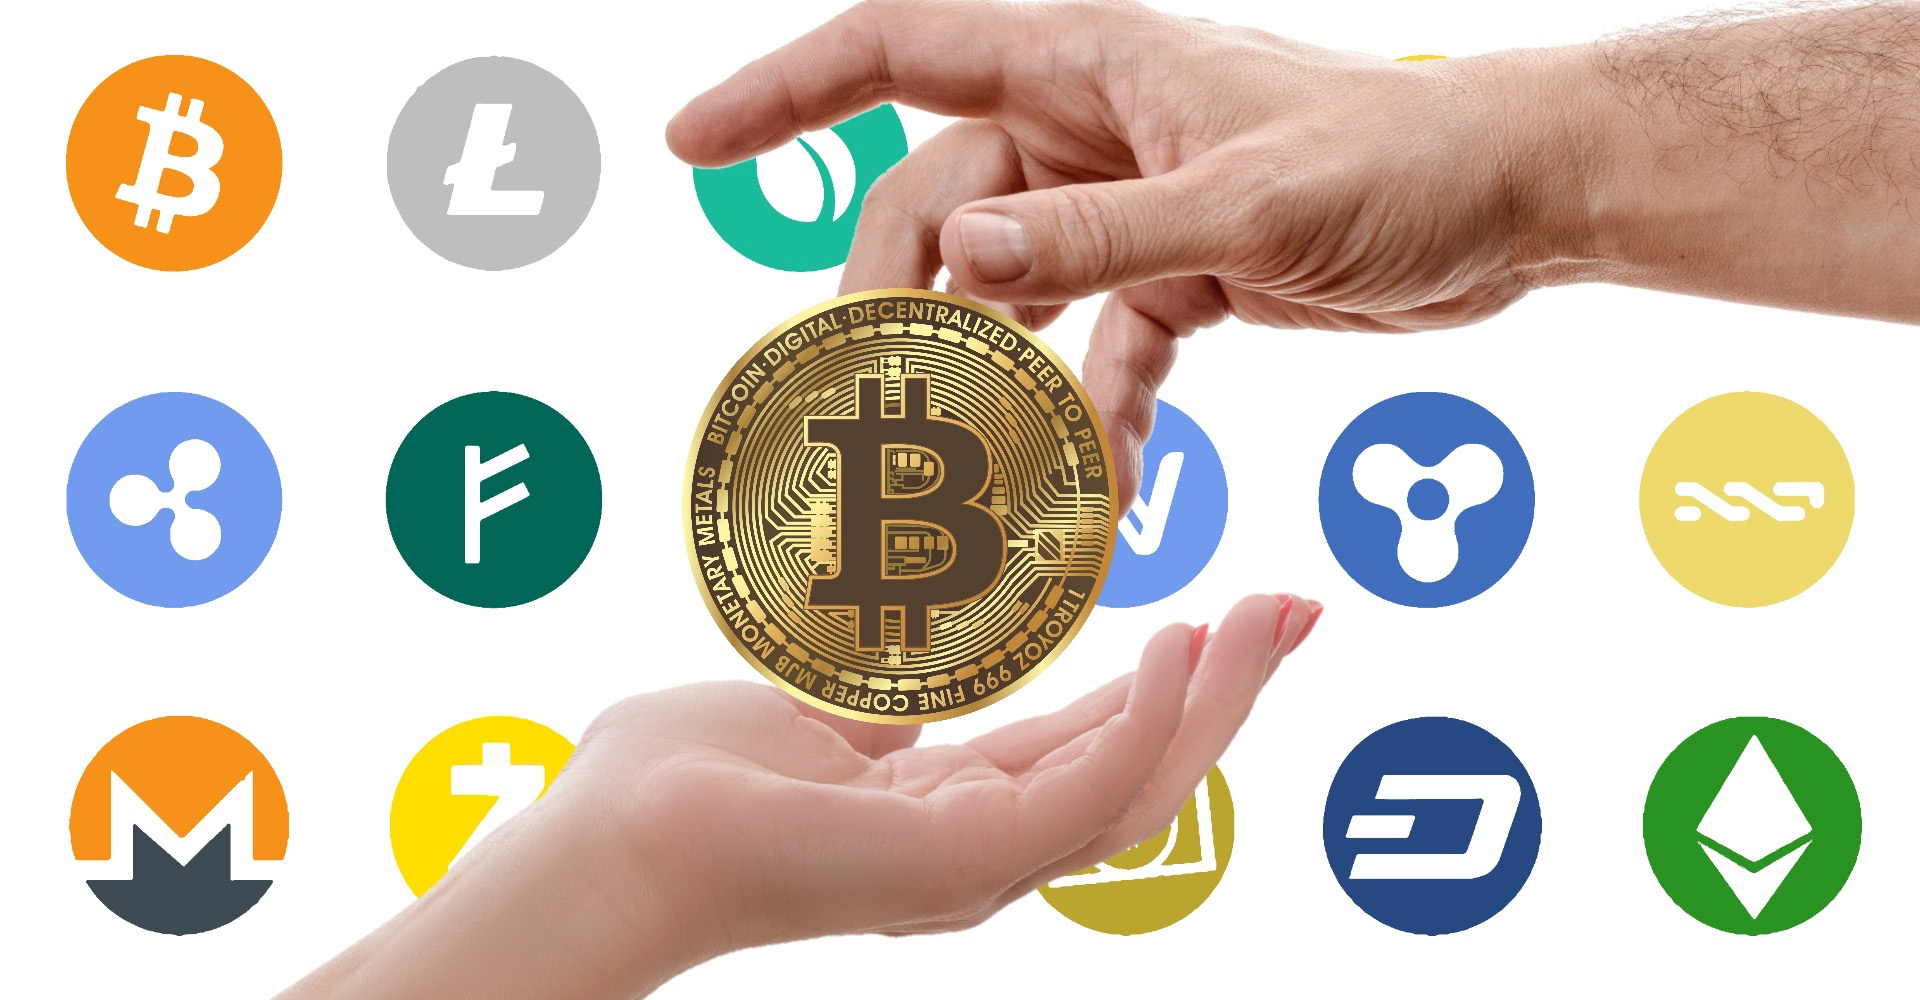
\includegraphics[width=\linewidth]{graphII-04-cryptocurrency-logos.jpg}}%
Dans un premier temps, on a pensé que la chaîne de blocs ne pouvait servir qu'à des applications de \gls{cryptographicmoney} --- au passage, on peut noter qu'il en existe à ce jour environ sept cents établies sur le modèle du \textit{bitcoin}, tellement l'idée a semblé intéressante, voire géniale.
Depuis quelques années on s'est aperçu que la \textit{blockchain} pouvait servir à bien d'autres choses, en s’appuyant sur le fait que ce fichier partagé est indestructible, par le nombre de copies et d'acteurs qui peuvent exercer un contrôle sur lui.

\paragraph{Cadastre} Ce n'est pas encore en place, mais on a envisagé de faire un cadastre à base de \textit{blockchains}. Les informations de propriété des terrains découpés seraient inscrites sur une \textit{blockchain}, dont seules certaines autorités auraient le droit d'aller inscrire des informations.

\sidegraphic[\textup{Blockchain} et cadastre ? Ici le champs de Mars et la tour Eiffel.]{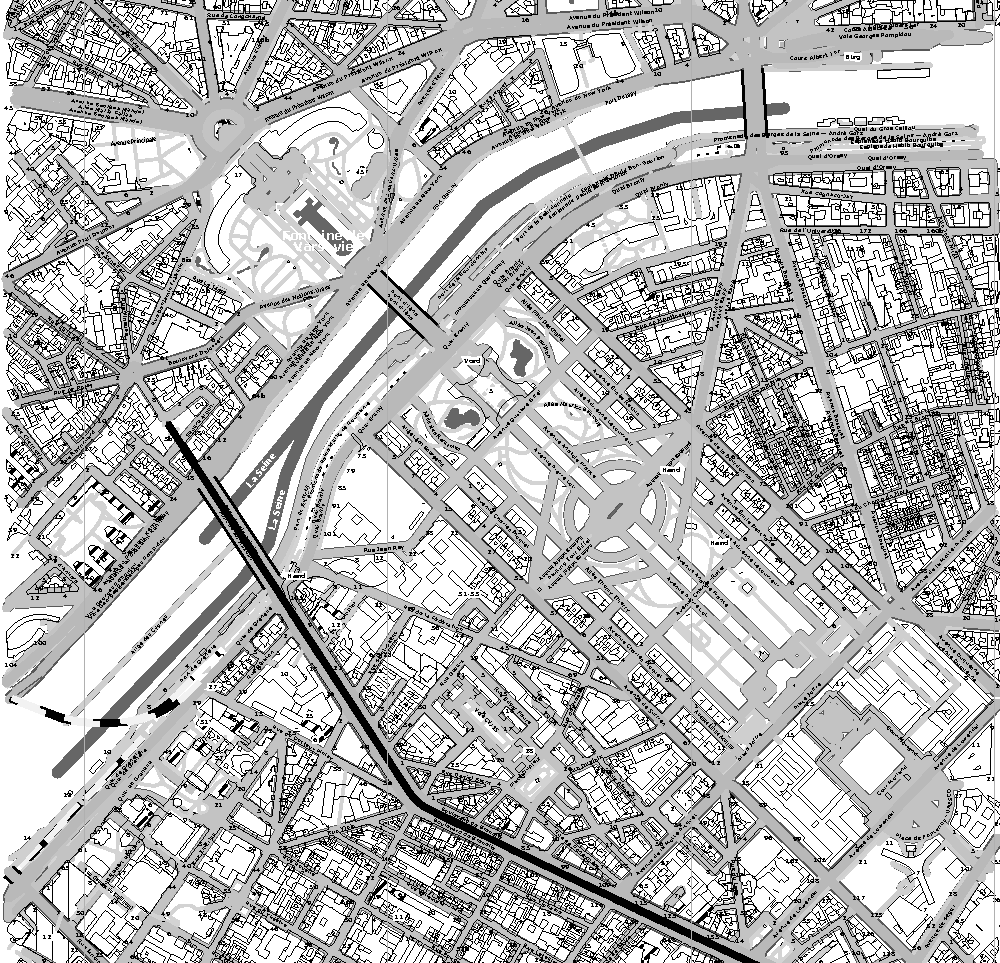
\includegraphics[width=\linewidth]{tour-eiffel-cadastre.pdf}}%
Quand une vente serait opérée, on écrirait une information, non pas en effaçant la précédente, mais en venant la compléter en indiquant que tel terrain a été vendu à un nouveau propriétaire. Cette information serait accessible à tous à partir du moment où elle serait multipliée et rendue indestructible par l'utilisation de primitives cryptographiques.

Simplement en se connectant à l'Internet, on pourrait connaître les biens immobiliers des propriétaires avec bien plus de fiabilité qu'un système centralisé. Cela permettrait d'établir une sorte de confiance vis-à-vis des données, notamment dans des pays où la corruption sévit ou dans lesquels le cadastre n'existe pas.

\paragraph{Véracité des diplômes} Une autre application potentielle concernerait les diplômes des écoles et des universités. Aujourd'hui, quand on veut savoir si quelqu'un possède un diplôme, c'est quasiment impossible ou alors il faut vérifier auprès de chaque université ou école qui a accordée ce diplôme.

\sidegraphic[\textup{Blockchain} et diplômes délivrés ?]{
\includegraphics[width=.75\linewidth]{graphII-06-diploma-symbol.pdf}}%
On peut imaginer une blockchain sur laquelle les établissements d'enseignement et de formation iraient indiquer les diplômes qu'elles délivrent, puis pour savoir si telle personne dispose effectivement de tel diplôme, chacun pourrait lire la blockchain. 
Là encore, la démultiplication du fichier garantirait la validité de l'information. 

Régulièrement, des gens proposent de nouvelles applications des \textit{blockchains}, donc d'une information partagée qui tient sa garantie de sûreté de par sa nature distribuée. Les développements en ce sens constituent une véritable révolution numérique, qui ne concerne pas uniquement les banques, mais également les organismes gouvernementaux et bien d'autres acteurs.

\overparagraph{Conséquences écologiques}

À propos du \textit{Bitcoin}, il est dit qu'il entraîne une dépense colossale d'énergie électrique et c'est vrai. La quantité d'électricité qui est dépensée pour faire fonctionner le protocole est énorme. Néanmoins, il faut bien comprendre pour l'avenir du développement des \textit{blockchains}, que cette particularité propre au \textit{Bitcoin} n'est pas générale. 

Dans leur ensemble, les \textit{blockchains} n'ont pas obligation d'avoir un système --- appelé système de minage du \textit{Bitcoin} --- qui entraîne une dépense importante d'électricité. C'est une erreur de croire que le développement des \textit{blockchains} va être freiné par ces considérations. 

%\printlocalglossary[-4pt]{9}
\printlocalglossary{9}

%\vspace*{-\baselineskip}
\subsection[\textit{Startups} bien de chez nous...]{\textit{Startups} \textit{Blockchain} bien de chez nous...}
\label{sub:II.3.2}

\begingroup\itshape
Le milieu des startups\caution[t]<firstcolor>{%
\upshape Texte de Serge \textsc{Abiteboul} et Pierre \textsc{Paradinas} publié sur \href{https://www.lemonde.fr/blog/binaire/2016/07/20/des-startups-blockchain-bien-de-chez-nous/}{Binaire} --- blog du numérique du journal \textsc{Le Monde} --- le 20 juillet 2016.}{\upshape Note de la rédaction}
 et des grandes entreprises d’informatique s’excite régulièrement sur un nouveau sujet. On voit défiler les modes à grande vitesse : \textup{big data}, Internet des objets, \textup{machine learning}... Et le petit dernier, la « \textup{blockchain} ». Nous allons parler ici de \textup{startups} françaises dans ce domaine. Nous allons supposer que le lecteur est vaguement familier avec la technologie \textup{blockchain}, comme expliqué, par exemple, dans l’\href{https://www.lemonde.fr/blog/binaire/2015/01/06/des-ordinateurs-au-dessus-des-attaques/}{article} de Jean-Paul \textsc{Delahaye} pour \textsc{Binaire}.
\endgroup

\sidegraphic{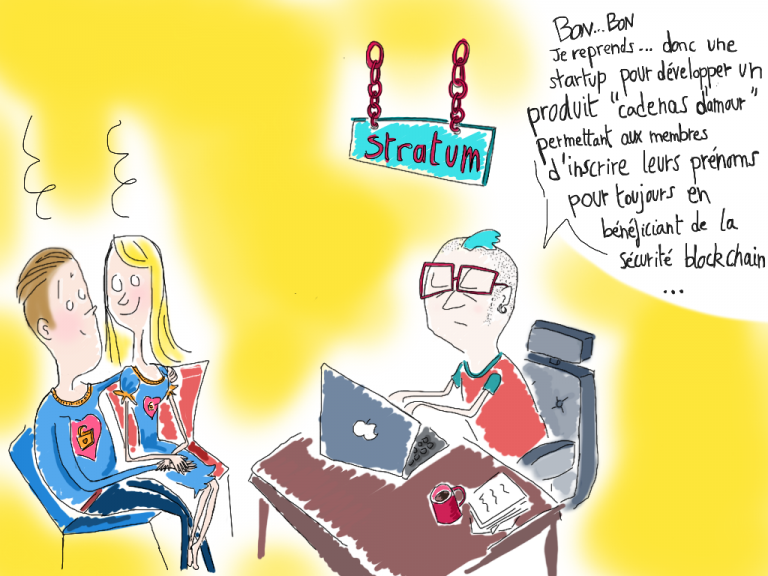
\includegraphics[width=\linewidth]{graphII-07-blockchain-amour.png}}{Laure \textsc{Cornu}}
Une \textit{blockchain} est un registre numérique public (sur le Web). Les données sont écrites dans un « grand livre » dont chaque ordinateur participant a une copie identique. On peut ajouter aux registres des transactions (au sens informatique comme au sens bancaire du terme) et ce, de manière totalement distribuée et sécurisée, assurant  l’intégri\-té de ces transactions. Les transactions sont réalisées l’une après l’autre. 

La \textit{blockchain} permet donc de concevoir des architectures véritablement décentralisées ; ce n’est pas simple parce que plusieurs transactions peuvent vouloir s’ajouter en même temps au registre et une seule doit y arriver. À chaque instant, la \textit{blockchain} contient tout l’historique des transactions. La technologie \textit{blockchain} est à l’origine d’une crypto-monnaie, le \textit{Bitcoin}, qui agite beaucoup les milieux financiers. Les \textit{Bitcoins} servent d’ailleurs eux-mêmes de « ressources » pour le fonctionnement des \textit{blockchains}. Les \textit{blockchains} semblent conduire à des échanges sécurisés distribués qui se libèrent du tiers de confiance (une banque centrale) ou d’une plateforme centralisatrice.

Cette techno n’est pas si vieille. L’an zéro du \textit{Bitcoin}, c’est 2008. Mais pourquoi tant d’intérêt soudain : sans doute en partie à cause du succès de \href{https://www.afternic.com/forsale/chain.com?utm_source=TDFS_DASLNC&utm_medium=DASLNC&utm_campaign=TDFS_DASLNC&traffic_type=TDFS_DASLNC&traffic_id=daslnc&}{\texttt{chain.com}}\caution[t]<secondcolor>{Lien mort au 31 juillet 2020.}{Attention !} qui, autour du \textit{Bitcoin}, propose une plateforme pour des échanges financiers entre entreprises. La technologie a mûri, ce que l’on observe également avec une plateforme \textit{open-source} de \textit{blockchain} très populaire, \href{https://en.wikipedia.org/wiki/Ethereum}{\textsc{Ethereum}}.

On notera d’abord des \textit{startups} autour des technologies financières comme \href{https://www.paymium.com/}{\textsc{Paymium}} (NdR --- associé à \href{https://blockchain.io/}{\textsc{blockchain.io}} depuis 2018) et \href{https://www.ledger.com/}{\textsc{Ledger Wallet}}. La première permet d’acheter et vendre des \textit{Bitcoins}, la seconde propose un portefeuille sécurisé sur \textit{smartcard} ou clé USB. Mais la techno \textit{blockchain} ouvre de nombreuses autres possibilités techniques, même si ses usages se cherchent encore.

\sidegraphic{
\includegraphics[width=.75\linewidth]{bitcoin-accepted-here-printable.png}}
Pour entrer dans ce nouveau domaine, il faut faire une distinction essentielle entre la \textit{blockchain} public ou privé. Dans le public, utilisé pour les \textit{Bitcoins}, chacun peut participer, par exemple en achetant ou en vendant des \textit{Bitcoins}. Dans le privé, pour participer, il faut être « approuvé » par une autorité. Les vraies nouveautés semblent venir plutôt du coté des \textit{blockchains} privées.

Une belle \textit{startup} pour commencer : \href{https://www.stratumn.com/}{\textsc{Stratumn}}. La techno \textit{blockchain} est compliquée. \textsc{Stratumn} va la proposer « \textit{as a service} ». On touche là à un des freins des \textit{blockchains} : c’est une techno encore jeune et les outils sont encore compliqués à utiliser. \textsc{Stratumn} essaie de les simplifier pour vous. Un beau programme. Vous venez avec votre idée d’application à coup de blockchain. Vous pouvez vous consacrer à cette application, \textsc{Stratumn} gère la techno.

Mais pour développer quelle application ? Là vous avez le choix. Vous avez \href{http://ledgys.io/}{\textsc{Ledgys}}\caution[t]<secondcolor>{Lien mort au 31 juillet 2020.}{Attention !} qui développe une place de marché sécurisée au dessus de la technologie \textit{blockchain} ou \href{https://belem.io/}{\textsc{Belem}} qui vise la gestion de données distribuées et la transmission d’informations sécurisée. Vous avez aussi \href{https://keeex.me/fr/}{\textsc{Keeex}} qui attaque le travail collaboratif avec encore de la gestion sécurisée de données décentralisées ou \href{https://www.woleet.io/}{\textsc{Woleet}}, qui s’intéresse à la propriété intellectuelle et la certification entre autres choses.

Elles sont trop nombreuses ces \textit{startups}. Il faudrait parler de \href{www.aedeus.com}{\textsc{aeDeus}}\caution[t]<secondcolor>{Lien mort au 31 juillet 2020.}{Attention !}, « la Première solution \textit{blockchain} 100\% française » (sic), ou de \href{https://www.kaiko.com/}{\textsc{Kaiko}} «~\textit{We organize Bitcoin’s information by making the tools businesses need to succeed in the uncharted world of Bitcoin, and blockchain technology} » (dans la version française de leur site).

Nous ne sommes pas certains d’avoir toujours compris ce que ces \textit{startups} faisaient. Certaines nous ont paru encore très préliminaires. D’autres \textit{startups} que nous avons regardées nous ont semblé bien trop fumeuses pour être mentionnées. Nous avons probablement raté de jolies perles. En tous cas, nous ressortons de cette balade dans les \textit{startups} françaises du \textit{blockchain} avec la sensation confuse qu’il est en train de se passer quelque chose, que si mille fleurs ne sont pas prêtes à surgir, quelques beaux bourgeons pourraient bien éclore.

\begin{gofurther}[before skip=12pt]
\begin{itemize}\jazzitem
\item \href{https://interstices.info/le-bitcoin-une-monnaie-100-numerique/}{Le \textit{bitcoin}, une monnaie 100\% numérique}, Rémy \textsc{Chrétien} et Stéphanie \textsc{Delaune}, \textsc{Interstices}, 8 septembre 2014 ;
\item \href{https://sciencetonnante.wordpress.com/2016/06/24/le-bitcoin-et-la-blockchain/}{Le \textit{Bitcoin} et la \textit{Blockchain}}, David \textsc{Louapre}, Science étonnante, 24 juin 2016 ;
\item \href{https://www.lemonde.fr/blog/binaire/?s=blockchain}{Série d'articles} publiés dans \textsc{Binaire} ;
\item \href{https://medium.com/cornell-tech/everything-you-always-wanted-to-know-about-icos-but-were-afraid-to-ask-b9728dc38b81}{\textit{Everything* You Always Wanted to Know About the Blockchain but Were Afraid to Ask}}, Arnaud \textsc{Sahuguet}, The Foundry @ Cornell Tech, 17 octobre 2017 ;
\item \href{https://www.frenchweb.fr/3-start-up-francaises-qui-innovent-avec-la-blockchain/239443#gsc.tab=0}{3 start-up françaises qui innovent avec la blockchain}, \textsc{FrenchWeb.fr}, 13 mai 2016 ;
\item \href{https://techcrunch.com/2015/10/03/the-blockchain-might-be-the-next-disruptive-technology/?ncid=rss&guccounter=1}{\textit{The Blockchain Might Be The Next Disruptive Technology}}, Florian \textsc{Graillot}, \textsc{Techcrunch}, 3 octobre 2015 ;
\item \href{https://piazza.com/princeton/spring2015/btctech/resources}{\textit{BTC-Tech: Bitcoin and Cryptocurrency Technologies}}, Princeton University, Spring 2015.
\end{itemize}
\end{gofurther}


%----------
\section[Numérique en question(s)]{Numérique en question(s)}
\label{sec:II.4}

Le numérique transforme en profondeur notre monde. Repérer ces transformations, comprendre les principes profonds du monde numérique et les changements de valeurs induits, pour mieux s'interroger sur notre devenir. Une invitation à revisiter les questions traditionnelles de la philosophie sous ce nouvel éclairage...

%\vspace*{-0.5pt}
\subsection[Penser le numérique]{Penser le numérique}
\label{sub:II.4.1}

L'ingénierie des connaissances et le \gls{semantic-web}\caution[t]<secondcolor>{%
\href{http://web-and-philosophy.org/abouta-propos/bio/}{Alexandre \textsc{Monnin}} est docteur en philosophie de l’Université Paris 1 Panthéon-Sorbonne où sa thèse portait sur la philosophie du Web \parencite{Monnin:2013}. Il est chercheur dans l'équipe \textsc{Inria} \href{https://www.inria.fr/fr/liste-des-equipes-projets}{\textsc{Wimmics}} et expert \textit{Open Data} auprès de la mission \textsc{Etalab} sous la responsabilité du Premier Ministre. Il a initié plusieurs projets mobilisant les technologies du Web de données, à l'instar du \textsc{DBpedia} francophone et de \textsc{Re-Source}, le système d'information de la Fondation des Galeries Lafayette pour l'art contemporain.}{À propos de l'intervenant}
 sont des disciplines, des outils technologiques qu'on utilise pour formaliser un certain nombre de domaines, lesquels n'appartiennent pas forcément aux champs scientifiques traditionnels, comme à titre d'exemple la banque. Il peut s'agir d'établir des \glspl{ontology} précises ou larges concernant des objets, des processus de travail et tout ce qui peut se formaliser à des fins d'informatisation.

\subsubsection[Ontologie]{Notion d'ontologie}
\label{subsub:II.4.1.1}

\overparagraph{Formalisation}

%Cette orientation 

Cette formalisation en contexte informatique a d'abord été porté par l'intelligence artificielle, en particulier avec les \glspl{expert-system}. L'idée est de disposer d'une \gls{data-modelling} d'un domaine afin, une fois cette étape réalisée, de permettre à des machines de produire des inférences, des raisonnements à partir des entités du domaine et de générer ainsi de nouvelles connaissances.

\begin{marginvideo}
	[\label{vid:II.6}Informatique et philosophie.]%
	\href{https://www.youtube.com/watch?v=sMXR1xUfLAo&list=PLWvGMqXvyJAMNWRvODUB5Ry3licACdaa0&index=16}%
		{
\includegraphics[width=\marginparwidth]{./Images/Pictograms/film-strip-dark-electric-blue.png}}%
	%\movie[width=\marginparwidth,showcontrols]%
	%	{
\includegraphics[width=\marginparwidth]{./Images/Pictograms/film-strip-dark-electric-blue.png}}%
	%	{./Videos/Chapter02/vidII-04-philosophy-HD.mp4}%
	\launchvideo{https://www.youtube.com/watch?v=sMXR1xUfLAo&list=PLWvGMqXvyJAMNWRvODUB5Ry3licACdaa0&index=16}
\end{marginvideo}

Le mot \emph{ontologie} est emprunté à la philosophie, introduit par John \textsc{McCarthy} le créateur de l'intelligence artificielle, à tout le moins l'initiateur de ce qu'on appelle l'\gls{logical-ai}. Il existe d'autres courants en IA, mais nous nous inscrivons ici dans celui-ci.

Le concept d'ontologie a une histoire complexe. Sans rentrer dans les détails, il désigne à la fois quand il apparaît, une théorie de l'objet et, sous sa forme popularisée, une théorie de ce qui existe. Ce mot a été adopté par John \textsc{McCarthy} pour indiquer ce qui existe à l'intérieur d'un domaine spécifique. On va donc procéder à la modélisation des données d'un domaine, de ses objets et de leurs relations entre eux comme mentionné plus haut.

\overparagraph{Philosophie et ontologies informatiques}

Le concept d'ontologie en philosophe est extrêmement important, essentiellement employé au singulier. L'informatique s'est approprié le mot avec l'idée qu'il y a \emph{des} ontologies puisque chacune est rattachée à un domaine différent.

Il existe donc deux acceptions selon la perspective que l'on adopte, considérant ainsi les ontologies informatiques comme des artefacts techniques. Néanmoins, même s'il y a une transformation importante du sens du concept d'une discipline à l'autre, des constantes demeu\-rent, notamment le fait qu'en informatique on va aller chercher des outils de la philosophie pour modéliser les domaines et ce qui s'avère exister dans un espace limité et parfois, lorsqu'on essaye d'agréger plusieurs domaines formalisés, faire appel à ce qu'on appelle des ontologies de haut niveau issues de la philosophie. Là encore, on à cette dernière emprunte des concepts permettant de décrire la réalité de manière très abstraite ; c'est le travail des ingénieurs des connaissances, qui apportent de quoi peupler ces concepts et finalement raccorder ces ontologies les unes aux autres.

D'ailleurs des philosophes travaillent désormais dans le champ des ontologies informatiques, comme par exemple Barry \textsc{Smith} qui se qualifie « d'ontologue » et non plus de philosophe. Toutefois ces travaux ne sont pas conduits comme en ingénierie des connaissances, mais sous couvert d'une approche de philosophe. Il est donc intéressant d'avoir ce dialogue et ce regard sans forcément adhérer de manière intégrale à une vision plutôt qu'à une autre. 


\subsubsection[Transformations]{Transformations des valeurs dans le monde numérique}
\label{subsub:II.4.1.2}

\begin{marginvideo}
	[\label{vid:II.7}Comment le monde devient numérique ? Gérard \textsc{Berry}, 2008.]%
	%\movie[width=\marginparwidth,showcontrols]%
	%	{
\includegraphics[width=\marginparwidth]{./Images/Pictograms/film-strip-dark-electric-blue.png}}%
	%	{./Videos/Chapter02/vidII-05-berry-20080117.mp4}%
	\href{https://www.college-de-france.fr/site/gerard-berry/inaugural-lecture-2008-01-17-18h00.htm}%
	  {
\includegraphics[width=\marginparwidth]{./Images/Pictograms/film-strip-dark-electric-blue.png}}%
	\launchvideo{https://www.college-de-france.fr/site/gerard-berry/inaugural-lecture-2008-01-17-18h00.htm}
\end{marginvideo}

Pour réfléchir à la notion de monde numérique, on peut partir de la formulation de Gérard \textsc{Berry} dans sa leçon initiale au Collège de France : « \href{https://www.college-de-france.fr/site/gerard-berry/inaugural-lecture-2008-01-17-18h00.htm}{Comment le monde devient numérique ?} ». Ce devenir avait été pointé par le chercheur en intelligence artificielle \href{https://en.wikipedia.org/wiki/Philip_E._Agre}{Phil \textsc{Agre}} qui remarquait que le numérique va formaliser puis rendre opérationnel un tas de domaines sans toutefois être toujours fidèle au domaine initial.

\overparagraph{Confiance, défiance, législation}

Ainsi, le numérique s'empare d'un certain nombre de concepts, de pratiques, de valeurs, il les formalise, il les opérationnalise, il les numérise tout simplement, mais ce faisant, il les transforme.

Pour illustrer le propos, il est possible de prendre en exemple la problématique de la confiance numérique. La confiance telle qu'elle est définie par les sociologues consiste à ne pas savoir quelque chose, elle est de l'ordre du non-­savoir tout en y portant crédit.

Si l'on confie son enfant à une nounou et que l'on met en place un dispositif avec des caméras qui la filment vingt-quatre heures sur vingt-quatre, la confiance envers la nounou est pour le moins absente... Donc on va avouer que le numérique ici, avec cette idée de surveillance, de générer des traces qui vont permettre de suivre tout ce qui se passe, n'est pas finalement un dispositif de confiance, mais en fait de défiance envers la nounou. Lui faire confiance serait : « je lui confie mon enfant, je ne sais pas ce qui se passe, mais j'accepte malgré tout de lui confier mon enfant ». 

D'une certaine manière, en opérationnalisant la confiance, on aboutit au résultat inverse : la défiance. Le numérique transforme donc les valeurs ou les entités qu'il opérationnalise et, parfois, les transforme en sens opposé de ce qu'elles étaient précédemment.

La loi peut également fournir un bon exemple. Il existe des ontologies juridiques pour essayer de comprendre et établir des raisonnements à partir du droit. Toutefois, une des évolutions importantes de ces dernières années est de voir la justice rendue \textit{a priori} en lieu et place d'un fondement normal du droit appliqué \textit{a posteriori}, à l'issue d'un procès, d'un jugement, etc. En effet, comme pour les guerres préemptives --- \textit{preemptive wars} ---, on assiste à une transformation du droit qui vise à prévenir un certain nombre de crimes ou de délits.

On va ainsi demander à des tiers, qui peuvent d'ailleurs être des entreprises, d'utiliser leurs algorithmes, leurs données, les données auxquelles elles ont accès concernant les personnes, pour justement permettre d'éviter qu'un certain nombre de crimes ou de conduites aient lieu. Donc, là aussi on a une transformation ; de l'\textit{a posteriori} à l'\textit{a priori}. L'\textit{a priori} juridique n'aurait eu aucun sens précédemment, mais outiller techniquement par le numérique, il tend à devenir la nouvelle norme. C'est là où c'est quelque chose qu'il faut vraiment essayer de penser : la manière dont le numérique non seulement transforme le monde --- le monde devient numérique ---, mais encore comment ce devenir change un certain nombre de pratiques et de valeurs. Ce faisant, il n'est pas certain que les valeurs nouvelles qui émergent soient celles dans lesquelles on se reconnaisse toujours. 

\overparagraph{Devenir et pérennité}

À l'énoncé de Gérard \textsc{Berry}, il faudrait rajouter une petite pastille. En effet, à y regarder de plus près, certes le monde devient numérique, mais il n'a pas les moyens de le rester.

C'est un point très important car le numérique n'est pas simplement de la science informatique, ce sont aussi des développements concrets, matériels, qui demandent des métaux, des ressources, de l'énergie, etc. Dans cette perspective, cela coûte finalement très cher de faire du numérique. À titre d'exemple, les outils de \textit{deep learning} qu'utilisent les grandes entreprises et les algorithmes qui sont mobilisés consomment énormément d'énergie, donc ce ne sont pas forcément des choses généralisables dans toutes les situations, ni toutes les circonstances. 

Ainsi, le monde devient numérique, il ne peut pas le rester et tout cela va en fait va très vite. Il ne faut pas simplement penser qu'on est dans une révolution et s'installer dans cette idée, d'une certaine manière qui peut être rassurante. Il y a une évolution, mais il faut se dire qu'on a affaire à une évolution qui est parallèle à d'autres évolutions, comme par exemple le changement climatique ou les perspectives d'effondrement dont on peut parler par ailleurs. Il va falloir penser tous ces éléments-là de concert, resynchroniser des futurs qui pour le moment ne le sont pas et qu'on ne sait pas exactement comment le faire. La question est de savoir que cette révolution numérique que nous vivons, ce devenir numérique du monde est lui-­‐même temporaire. Il faut d'ors et déjà penser la 
fin du numérique en parallèle d'autres modèles. Ainsi, ces cultures numériques sont en partie temporaires et c'est ça qui est très difficile aujourd'hui à penser.

\overparagraph{Héritage et liens au monde réel}

C'est dans l'expression « monde numérique » qu'il faut peut-être chercher des pistes de réflexion face aux problématiques mentionnées, notamment parce que le lien entre le monde et le numérique ne va pas du tout de soi. On peut considérer que justement le monde n'est pas \textit{a priori} numérique, il n'est pas discret, il n'est pas \gls{digital}. La production du monde numérique représente un investissement considérable ne serait-ce qu'en termes de matériel, donc dire que le monde devient numérique implique aussi de longs et coûteux processus.

Ainsi, se dessine ici une dialectique à penser entre un monde qui devient numérique\sidenote{Quel est-­il, ce monde qui devient numérique ?} et l'Ancien\sidenote{Qu'est-ce que nous gardons ? Qu'est-ce que nous abandonnons ?} monde. Il y a donc une question d'héritage qui se pose au cœur de ce devenir numérique. De plus, si on considère que le monde ne peut pas rester numérique, nous devons penser l'héritage propre à ce monde numérique en deuxième surcouche. Là encore, que faut-il laisser de coté ? Ce sont là les véritables questions d'avenir et en particulier pour les jeunes générations.


\printlocalglossary{10}

\subsection[Être et écran]{Être et écran : changement de la perception}
\label{sub:II.4.2}

\sidegraphic[Stéphane Vial, PUF, 2013 \parencite{Vial:2013}]{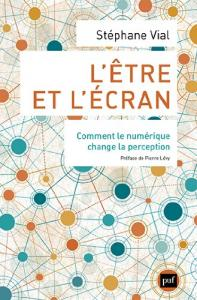
\includegraphics[width=\linewidth]{graphII-08-etre-ecran.jpg}}
« À tous ceux qui se demandent ce qu’il faut faire de la révolution numérique, il est facile de répondre d’un mot : il faut en faire le design ». Stéphane \textsc{Vial}, ancien philosophe enseignant à l’école Boulle, ne prêche pas seulement pour sa paroisse --- le « design numérique~», prolongement du design classique adapté aux systèmes interactifs, cherchant à donner « vie » à des usages et « forme » à des contenus informatisés ---, il s’inquiète plus fondamentalement des effets de la révolution en cours depuis trois décennies.

Il rappelle ainsi, par exemple, qu’entre 1981 et 2010 le nombre de terminaux interconnecté est passé de 213 à... 5 milliards. Et, pour figurer l’accélération fulgurante de ces évolutions, il souligne qu’en deux ans, entre 2010 et 2012, \textsc{Apple} a vendu autant de tablettes \textsc{iPad} que d’ordinateur \textsc{Macintosh} en vingt-quatre ans, soit 64 millions d’unités. Mieux, 120 millions étaient vendus en 2013 !

De quoi cette révolution est-elle le nom ? D’un bouleversement des conditions de perception du monde qui nous entoure, avec lequel on interagit, selon Stéphane \textsc{Vial}. En clair, il faut désormais, quoi qu’on fasse, en passer par les « interfaces » (\textit{e-mail}, \textsc{Facebook} et écrans en tous genres).


\overparagraph*{« Définir à nouveaux frais le concept de virtuel »}

S’inspirant de \textsc{Bachelard} et de sa « phénoménotechnique » --- étude des effets de la technique sur la perception et les modalités d’apparition des phénomènes ---, il conçoit le néologisme « ontophanique », pour rendre compte de ce qui se donne et apparaît à travers les interfaces numériques. Dénombrant les qualités de ce phénomène numérique, il définit du même coup à nouveaux frais le concept de « virtuel », trop marqué par un imaginaire métaphysique l’opposant au réel et l’assimilant à celui de néant. Or le virtuel n’est pas le néant. Et, s’il en est un aspect, il ne résume pas le phénomène numérique.

Bref, la question ne se situe pas entre l’être et le néant, mais bien entre l’être et l’écran ou, avec l’être et l’écran. Cet effort de définition compte parmi les plus heureux de ce travail de recherche qui donne de la matière et du corps à une réalité numérique trop souvent et paresseusement conçue comme un monde irréel et vaporeux, sinon fumeux.

\overparagraph*{« Le monde numérique participe de notre monde »}

Stéphane \textsc{Vial} le martèle : le monde numérique participe de notre monde et ses effets sont tout aussi palpables. Comment ne pas voir que les réseaux sociaux, \textsc{Twitter}, \textsc{Facebook}, nos « ordinateurs mobiles~» que sont désormais nos téléphones, les boîtes mail ou le développement des outils de réalité augmentée modifient notre environnement perceptif, participant à une « situation interactive généralisée » ?

Pour le chercheur, il convient donc d’exiger « du sujet contemporain un véritable travail phénoménologique en vue d’apprendre à percevoir cette nouvelle catégorie d’étants, les êtres numériques […]. Percevoir à l’ère numérique, c’est être contraint de renégocier l’acte de perception lui-même ».
Comment le renégocier ? En acceptant, selon le vœu de Gilbert \textsc{Simondon}, réinvesti par Stéphane \textsc{Vial}, d'accorder « aux objets techniques une place dans le monde des significations », en s'entendant sur le fait que « les objets font le monde ». Le design a de beaux jours devant lui.

\begin{gofurther}[before skip=12pt]
\textttl{Philosophie et numérique}
\begin{itemize}\jazzitem
\item \href{https://eduscol.education.fr/philosophie/actualites/archives/archives-actualites-2016/penser-le-numerique-une-question-philosophique}{Penser le numérique : une question philosophique ?}, Paul \textsc{Matthias}, conférence  du 1er décembre 2016 ;
\item \href{https://www.college-de-france.fr/site/gerard-berry/inaugural-lecture-2008-01-17-18h00.htm}{Pourquoi et comment le monde devient numérique}, Gérard \textsc{Berry}, conférence au Collège de France, 17 janvier 2008 ;
\item \href{https://www.youtube.com/watch?v=ZCBB0QEmT5g}{Les nouvelles technologies : révolution culturelle et cognitive} Michel \textsc{Serres}, conférence sur les nouvelles technologies lors du 40\frup{e} anniversaire de l'\textsc{Inria} , 2007 ;
\item \href{http://maisouvaleweb.fr/la-societe-des-calculs-sous-la-loupe-de-la-sociologie-a-quoi-revent-les-algorithmes-dominique-cardon-lecture/}{La société des calculs sous la loupe de la sociologie – A quoi rêvent les algorithmes}, Dominique \textsc{Cardon},  Mais où va le web ?  P(a)nser le numérique, article publié le 14 février 2014 ;
\item \href{https://interstices.info/ontologies-informatiques/}{Ontologies Informatiques}, Fabien \textsc{Gandon}, \textsc{Interstices}, article publié le 22/05/2006 ;
%\item \href{https://hal.archives-ouvertes.fr/hal-00769665}{Le sens de la technique : le numérique et le calcul}, Bruno \textsc{Bachimont}, Encres \textsc{Marines}, Les Belles Lettres, pp.191, 2010.
\end{itemize}
%\vspace*{2pt}
%\textttl{Colloque}
%\begin{itemize}\jazzitem
%\item \href{https://eduscol.education.fr/philosophie/actualites/archives/archives-actualites-2016/philonum-2016}{\#{PhiloNum}}, colloque du 16 au 20 janvier 2017, Centre Georges Pompidou,  \textsc{Eduscol}, article publié le 23/12/2016.
%\end{itemize}
\vspace*{2pt}
\textttl{Impact écologique du numérique}
\begin{itemize}\jazzitem
\item \href{https://ecoinfo.cnrs.fr/2015/12/23/les-effets-rebond-du-numerique/}{Les effets rebond du numérique}, Cédric \textsc{Gossart}, \textsc{EcoInfo}, article publié le 23/12/2015 ;
%\item \href{http://www.e-rse.net/technologie-ecologie-environnement-solution-19779/#gs.DyVsDac}{La technologie peut-elle résoudre les problèmes environnementaux ?} Clément \textsc{Fournier},  \textsc{E-RSE.net}, publié le 11 mai 2016.
\end{itemize}
\vspace*{2pt}
\textttl{Web sémantique}
\begin{itemize}\jazzitem
\item \href{https://www.canal-u.tv/producteurs/inria/cours_en_ligne/web_semantique_et_web_de_donnees}{\textsc{Mooc} Web Sémantique et Web de données}, Fabien \textsc{Gandon}, Olivier \textsc{Corby} et Catherine \textsc{Faron Zucker}, \textsc{Inria} 2015 Canal-U.
\end{itemize}
\end{gofurther}



%----------
\section[Que faire de ces ressources ? Quiz]{Que faire de ces ressources ? Autoévaluation}
\label{sec:II.5}

\vspace*{-4pt}
Les questions\caution[b]<thirdcolor>{%
La présentation des quiz du document\linebreak suit plus ou moins celle de la platefor\-me \textsc{Fun-Mooc}. La fonctionnalité manquante --- pas encore implémentée dans l'extension de style \LaTeX{} usitée --- est relative à la comptabilisation des points et à leur enregistrement. Aussi, il appartient au lecteur de jouer le jeu dans l'auto\-évaluation de ses connaissances.}{Note de la rédaction}
à choix multiple\parnote{De manière traditionnelle en \textsc{Ihm}, lorsqu'une seule réponse est correcte, les propositions sont précédées d'un cercle à cocher (\emph{radio button}) ; en revanche, dans le cas de plusieurs solutions, il s'agit de carrés (\emph{check box}).}
--- QCM --- qui sont à suivre clôturent le présent chapitre \qnameref{chap:II}. 
L'explication des réponses correctes s'affiche en marge : bouton « Afficher la réponse ».
\parnotes

\vspace{6pt}

\begin{quiz}[title={Web et usages}]
\vspace{-\baselineskip}
\begin{quizquestion*}[b]{2}{1}{Application de courrier électronique}
<Le courrielleur et le Web sont des applications d'Internet. Il est certes possible de consulter ses couriers électroniques depuis une interface Web mais le courriel est une technologie différente au même titre que la téléphonie OIP.>
Le courrier électronique est une application du Web.
\points{1}
	\mcqproposal{Vrai.}
	\mcqproposal{Faux.}
\end{quizquestion*}

\begin{quizquestion*}[c]{2}{1,3}{Notion de réseau social}
<La notion de réseau est connue depuis bien avant le Web : chaque vendeur a son réseau de clients et de fournisseurs, chaque homme ou femme politique ne peut survivre sans un réseau, nous avons tous un réseau d'amis ou encore associatif. Les sciences humaines et sociales étudient ces phénomènes depuis fort longtemps. Avec la numérisation de ces réseaux, la science informatique peut développer et exploiter des méthodes puissantes pour décupler la portée de ces analyses.>
Depuis quand existent les réseaux sociaux ?
\points{1}
	\mcqproposal{Depuis la naissance d'Internet.}
	\mcqproposal{Depuis la naissance de \textsc{Facebook}.}
	\mcqproposal{Depuis (presque) toujours. L'humain est un être social qui n'a pas attendu Internet pour construire son réseau.}
\end{quizquestion*}

\begin{quizquestion*}<tooltip>[b]{2}{1,3}{Influence au sein d'un réseau}
<La centralité d'intermédiarité mesure la centralité du sommet d'un graphe, autrement dit, le nombre de fois où une personne est sur le plus court chemin entre deux autres nœuds, à quel point elle est intermédiaire et on passe par elle pour connecter deux autres personnes.
Un graphe orienté est un type de graphe qui permet de matérialiser le sens des relations entre deux nœuds.
La matrice d'adjacence est une autre manière de représenter un réseau.>
Qu'est-ce qui peut aider à déterminer la personne la plus influente au sein d'un réseau ?
\points{1}
	\mcqproposal{Un graphe orienté.}
	\mcqproposal{La centralité d'intermédiarité.}
	\mcqproposal{Une matrice d'adjacence.}
\end{quizquestion*}

\begin{quizquestion}[b]{1,3}{2,4}{Informatique dans les nuages}
<Si on gagne en sûreté et on diminue les coût de gestion informatique en externalisant les services, il faut comprendre que les données et calculs sont centralisés dans de gigantesques centres, hors de notre contrôle et l'impact environnemental est augmenté du fait des transmissions d'informations à travers la planète et des redondances matérielles pour garantir le bon fonctionnement.>
Quels sont les avantages principaux de l'utilisation du Cloud ?\\ Cocher les deux réponses exactes.
\points{1}
	\mcqproposal{Plus de sûreté car mes données sont stockées de manière redondante dans des centres bien sécurisés.}
	\mcqproposal{Moins d'impact environnemental puisque les machines ont été regroupées pour mutualiser leur gestion.}
	\mcqproposal{La possibilité d'accéder à des services informatiques même pour une entreprise qui n'a pas la compétence en interne.}
	\mcqproposal{C'est vraiment dans l'esprit d'Internet de décentraliser les données et les calculs.}
\end{quizquestion}

\begin{quizquestion}[c]{1,3}{2,4}{Monnaies cryptographiques}
<Effectivement, toutes sortes de contrats (achats de biens, accords entre structures, etc.) de manière certifiée peuvent être enregistrés dans le journal d'une \textit{blockchain}, y compris une action issue d'une personne unique. En revanche, l'identité de la personne ne peut être révélée par ce mécanisme.>
À quoi pourrait servir la \textit{blockchain} au delà de son usage pour les monnaies cryptographiques ?\\
Cocher les 2 réponses plausibles.
\points{1}
	\mcqproposal{Enregistrer toute sorte de contrats (achats de biens, accords entre structures, etc.) de manière certifiée.}
	\mcqproposal{Prouver l'identité d'une personne qui fait un acte.}
	\mcqproposal{Prouver l'antériorité d'une création : œuvre artistique, invention technique, etc.}
	\mcqproposal{Faire le café.}
\end{quizquestion}

\begin{quizquestion*}[b]{2}{1,3}{Blockchain et écologie}
<Le mécanisme de blockchain pose véritablement un problème écologique car la méthode repose sur une augmentation progressive des calculs pour garantir la sécurité des échanges donc de plus en plus d'énergie consommée.>%\\
Quant au calcul quantique son seul point commun avec le nucléaire et d'en partager les notions de physiques théorique.>
En quoi le mécanisme de blockchain pose-t-il un vrai problème écologique ?
\points{1}
	\mcqproposal{Il n'en pose aucun bien au contraire puisque les calculs sont distribués, cela répartit la consommation.}
	\mcqproposal{La méthode repose sur une consommation d'énergie de plus en plus importante pour sécuriser les échanges.}
	\mcqproposal{C'est à cause de l'aspect quantique des calculs, cela génère une vraie pollution nucléaire.}
\end{quizquestion*}

\begin{quizquestion}[c]{1,4}{2,3}{Numérique et philosophie}
<Le propos d'Alexandre \textsc{Monnin} explique que la confiance, philosophiquement centrée sur le non-savoir, devient avec le numérique une opérationnalisation de la défiance. Par ailleurs, les algo\-rithmes et leur capacité à traiter des données, favorise un droit préemptif qui vise à prévenir \textit{a priori} un crime plutôt qu'à le juger \textit{a posteriori}. Les deux autres notions ne sont pas évoquées par Alexandre \textsc{Monnin}, mais la liberté est au centre des questions qui se posent dans la section « Aspect légaux, économiques et éthiques du logiciel~» par Daniel \textsc{Le Métayer} ou Philippe \textsc{Lhardy}, ainsi que dans la section « Impact sociétal de la robotique » par Jean-Pierre \textsc{Merlet}, et la beauté est indissociable de l'art, que le cours évoque dans la section « Informatique et arts ».>
Quelles notions philosophiques le numérique transforme-t-il ?\\
Cocher les deux notions évoquées par Alexandre \textsc{Monnin}.
\points{1}
	\mcqproposal{La loi.}
	\mcqproposal{La beauté.}
	\mcqproposal{La liberté.}
	\mcqproposal{La confiance.}
\end{quizquestion}

\end{quiz}


\vfill\pagebreak\thispagestyle{empty}
